\documentclass[12pt,a4paper, oneside]{report}

\usepackage{style/cs}
\usepackage[a4paper, margin=1in]{geometry}

\usepackage{times}
\usepackage{graphicx}
\usepackage{latexsym}
\usepackage{amsmath,amsbsy}
\usepackage{amssymb}
\usepackage[matrix,arrow]{xy}
\usepackage{ae,aecompl}
\usepackage{amstext}
\usepackage{graphics}
\usepackage{ae,aecompl}
\usepackage{algorithm}
\usepackage{algorithmic}
\usepackage{color}
\usepackage{listings}
\usepackage{xcolor}

\usepackage{tabularx}

\usepackage{hyperref}

\usepackage[english]{babel}
\usepackage{pgfpages}

\usepackage{ucs}
\usepackage[utf8]{inputenc}
\usepackage[T1]{fontenc}

\usepackage{ifpdf}

\usepackage{xurl}
\usepackage{subcaption}

% yoinked from: https://tex.stackexchange.com/a/732867/301747
\lstdefinelanguage{json}{
    breaklines=true,
    showstringspaces=false,
    string=[db]{"},
    stringstyle=\color{green!50!black},
    morestring=[s][\color{black}]{\ \ "}{":},
    keywordstyle=\color{blue},
    keywords={true,false,null},
    literate=
     *{0}{{{\color{red}0}}}{1}
      {1}{{{\color{red}1}}}{1}
      {2}{{{\color{red}2}}}{1}
      {3}{{{\color{red}3}}}{1}
      {4}{{{\color{red}4}}}{1}
      {5}{{{\color{red}5}}}{1}
      {6}{{{\color{red}6}}}{1}
      {7}{{{\color{red}7}}}{1}
      {8}{{{\color{red}8}}}{1}
      {9}{{{\color{red}9}}}{1}
      {.}{{{\color{red}.}}}{1}
      {:}{{{\color{gray}{:}}}}{1}
      {,}{{{\color{gray}{,}}}}{1}
      {\{}{{{\color{gray}{\{}}}}{1}
      {\}}{{{\color{gray}{\}}}}}{1}
      {[}{{{\color{gray}{[}}}}{1}
      {]}{{{\color{gray}{]}}}}{1},
}


\graphicspath{{figures/}}
\ifpdf
  \DeclareGraphicsExtensions{.pdf,.jpeg,.png}
\else
  \DeclareGraphicsExtensions{.eps}
\fi

\centerchapter
\singlespace

\renewcommand{\thesisauthor}{Roland BÁLINT}
\renewcommand{\thesismonth}{September}
\renewcommand{\thesisyear}{2026}
\renewcommand{\thesistitle}{\app{}: a TPM-secured TOTP authenticator app running on a USB stick}
\renewcommand{\thesissupervisor}{Conf. dr. ing. Ciprian Pavel OPRIȘA}
\newcommand{\utcnlogo}{
\includegraphics[width=14.5cm]{img/tucn.jpg}}
\newcommand{\department}{\textbf{FACULTY OF AUTOMATION AND COMPUTER SCIENCE}\\
\textbf{COMPUTER SCIENCE DEPARTMENT}\\}

\newcommand{\app}{Authenstickator}
\renewcommand{\t}[1]{\texttt{#1}}
\renewcommand{\i}[1]{\textit{#1}}
\renewcommand{\b}[1]{\textbf{#1}}

\lstset{
    basicstyle=\footnotesize\ttfamily,       % Monospace font
    backgroundcolor=\color{gray!5},  % Light grey background
    frame=single,                     % Draws a box around the code
    rulecolor=\color{black!10},       % Light grey border
    breaklines=true,                  % Wraps long lines of code
    showstringspaces=false
}



\begin{document}

\begin{titlepage}
\vspace*{-2cm}
\utcnlogo
\begin{center}
\department

\vspace{5cm}

\Large {\textbf\thesistitle \\}
\vspace {1cm}
\large {MASTER'S THESIS}\\

\vspace{8cm}

\begin{tabularx}{\textwidth}{r l}  
Master graduate:   &  \textbf\thesisauthor \\
 & \\
Supervisor:  & \textbf\thesissupervisor \\
\end{tabularx}

\vspace{2.5cm}

\thesismonth, \thesisyear
\end{center}
\end{titlepage}

\begin{titlepage}
\vspace*{-2cm}
\utcnlogo
\begin{center}
\department

\vspace{1cm}

\newcolumntype{R}{>{\raggedleft\arraybackslash}X}%
\begin{tabularx}{\textwidth}{lR}
DEAN, & HEAD OF DEPARTMENT, \\
\textbf{Prof.Dr.Eng. Vlad MUREȘAN} & \textbf{Prof.Dr.Eng. Rodica POTOLEA}\\
\end{tabularx}

\vspace {2.5cm}

Master graduate:  \textbf\thesisauthor
\vspace{1cm}

\large \textbf\thesistitle \\
\vspace {1cm}

\end{center}


\begin{flushleft}
\begin{enumerate}
\item \textbf{Project proposal}:
  This thesis proposes a framework for running TOTP authenticator apps (the ones which provide six-digit codes as a second factor of authentication) on external devices like USB sticks, with the goal of replacing personal mobile devices.
  Then, it aims to showcase an implementation of the proposed framework, as a proof of concept.

 \item \textbf{Project contents}:
  Introduction, Objectives of the Research, Bibliographic Research, Project Presentation, Theoretical and Experimental Results, Conclusions.

 \item \textbf{Place of documentation}:
  Technical University of Cluj-Napoca, Computer Science Department

 \item \textbf{Consultants}:
 Conf. dr. ing. Ciprian Pavel OPRIȘA

 \item \textbf{Date of issuing the proposal:} November, 2025

 \item \textbf{Date of delivery:} September 6th, 2026
\end{enumerate}

\end{flushleft}

\vspace{3cm}

\begin{center}
\newcolumntype{R}{>{\raggedleft\arraybackslash}X}%
\begin{tabularx}{\textwidth}{X X}  %{lR}
 & Master's graduate: \dotfill \\
 & \\
 & Supervisor: \dotfill \\
\end{tabularx}



\end{center}

\end{titlepage}


% \include{declaratie}

\begin{titlepage}
\phantom{1}
\end{titlepage}

\newenvironment{definition}[1][Definition.]{\begin{trivlist}
\item[\hskip \labelsep {\bfseries #1}]}{\end{trivlist}}

\pagenumbering{roman}
\setcounter{page}{1}

\tableofcontents
\newpage

\clearpage
\newpage

\pagenumbering{arabic}
\setcounter{page}{1}

\chapter{Introduction}

``Digital security is the computer equivalent of disaster insurance.
Few people care very much about it or give it much thought, and everyone hates paying for it… until a catastrophe hits.
Then we are either really glad we had it or really sad that we didn't have enough of it or didn't have it at all.''\cite{tpmbook}.

In an ideal world, there would be no malicious actors, no hackers, and cybersecurity would not need to exist.
But we live in a world where cyberattacks are a daily phenomenon, yet companies, and people in general, keep choosing convenience over security.
Now that we live in ``the age of AI'', it seems like everyone is on a hunt for personal data, from hackers to big tech companies.
We barely started to understand that the internet is not a safe place, yet we find ourselves in a world where attackers are always one step ahead.
I hope that people slowly bypass their ``what do I have to hide?'' era, and start taking measures for their digital security.

There are clear measures, but they are usually inconvenient.
It is hard to make something hard for an attacker, but frictionless for the user.
Passwords are still the most common authentication and authorization method, although they have been proven inefficient since their birth.
We can see more and more companies enforcing two-factor authentication (2FA) on the users of their applications.
This way, the password gets paired with, for example, something the user has.
Now the black hat has to steal your phone as well, not just guess your dog's name and year of birth.

Digital good practices involve choosing security measures like 2FA, but not only.
One ground rule should be: never use company devices for personal use, and vice versa.
If each employee used their work laptop for work only, probably the phishing statistics would look better as well.
And yet, things get mixed very early on: you start to work at company Y (to avoid the saying X), and the first thing is that you get an account which needs a mobile authenticator app registered.
You pull out your phone, scan the QR code, and now you have your personal device coupled with your work life.

This coupling is a light one, but my thesis tries to break it.
I will present you an alternative to regular authenticator apps, which does not use your personal device.
And as long as you follow my guidelines, it won't be less secure.


\chapter{Objectives of the Research}

The objective of this thesis is to present a framework for running TOTP-based authentication apps on USB sticks without breaking 2FA principles, and showcase a proof of concept implementation of the framework called \app{}.

Many applications require you to enable two-factor authentication, and the most common option is to use an authenticator app.
In some cases you might want to avoid using your phone for such purposes.


\chapter{Bibliographic Research} \label{lab:ch3-bibliographic-research}

This chapter will go through the main ideas, principles, algorithms, and notions used throughout the implementation of \app{}.
They will be presented as found in literature, with references to bibliographic sources, hence the chapter's title.
While the sections don't necessarily come in a given order, I tried to structure them from the main ideas to the more detailed aspects.
Each section can be read in isolation, so feel free to jump to the one of your interest.



\section{Existing Solutions}

In this section I will present software solutions (sometimes backed by hardware) which solve a similar problem to what \app{} aims to solve.
They will be presented in comparison with \app{}, so you will see both arguments for and against my solution.
Frankly, I found no other project doing exactly what I do, so none of the presented solutions will be a one-to-one match to my project.
Also, when comparing, keep in mind that \app{} is developed by a single person, in a limited amount of time, and serves more as a proof of concept rather than a polished end product.

Without further ado, lets dive deep into the ``opponents'' of \app{}.



\subsection{YubiKey} \label{lab:c3-yubikey}
The YubiKey is a product if the company called yubico.
It has gained rising popularity over the last few years, both for personal and professional use.
It comes in various shapes and forms, but mostly resembles a USB stick.
However, these are custom-built hardware designed specifically to support different protocols which need a security key.

Citing from their website \cite{yubikey},
``The YubiKey works with hundreds of enterprise, developer and consumer applications, out-of-the-box and with no client software.
Combined with leading password managers, social login and enterprise single sign on systems the YubiKey enables secure access to thousands of online services.''
Their products also support OTP:
``OTP supports protocols where a single use code is entered to provide authentication.
These protocols tend to be older and more widely supported in legacy applications.
The YubiKey communicates via the HID keyboard interface, sending output as a series of keystrokes.
This means OTP protocols can work across all OSs and environments that support USB keyboards, as well as with any app that can accept keyboard input.''

Their most recommended product is YubiKey 5, and they call it the world's number one multiprotocol security key.
From these series, as of August 21st, 2026, the cheapest for 70.18 EUR.
Other models from this series go even more expensive, with the biggest price being 102.85 EUR.
The models differ in capabilities, but also physical size, the smaller ones costing generally more.

Yubico is a generally trusted company with a good reputation.
It is based in Stockholm, Sweden, and was founded in 2007 by Stina Ehrensvard.
According to Tracxn\footnote{\url{https://tracxn.com/d/companies/yubico/__fgcOVhxhBthY3y9De52Otl021ENbj9VtVBf2Ho1uoOI\#about-the-company}}, it is ranked 1st among its competitors.
They have around 300 employees and have a total of 30M USD funding.
However, the software that runs in YubiKey is closed-source.
They did have some security issues in the past\footnote{\url{{https://en.wikipedia.org/wiki/YubiKey\#Security_issues}}}, including:
\begin{itemize}
    \item \b{ROCA vulnerability - October 2017}.
        A vulnerability which affected many security keys which implemented RSA.
        It allowed an attacker to reconstruct the private key by using the public key.
        Yubico gave free replacements with newer series devices.
    \item \b{OTP password protection - January 2018}
        This affected a specific model, the YubiKey NEO.
        The password protection for the OTP functionality could be bypassed.
        Yubico offered a firmware update and free replacements.
    \item \b{Cloning vulnerability - September 2024}
        It allowed a person to clone a YubiKey if they gave physical access.
        It was remediated through a firmware update.
        This required advanced cryptographic and technical knowledge: they looked at the electromagnetic emissions of the keys. \cite{eukleak}
\end{itemize}

In comparison with \app{}, YubiKeys are much more secure, since they are specialized hardware.
It is backed by a stable company with a team of software and hardware engineers.
It went through various iterations, and leads in the domain of security keys.
They are a solution for various problems, OTP being just one tiny functionality of theirs.
They are widely used, also by big corporations.

In defense of my project, \app{} also has some benefits compared to a YubiKey.
First, the price of \app{} is bond to the price of the USB key it is used on, which is minuscule compared to 70 EUR.
Most of us have a spare USB stick laying around without a purpose, and with \app{}, we can give life to a potential electronic waste.
Second, the source code of \app{} is fully open source, so anyone can audit it or reuse it (respecting its GPL-3.0 license).
\app{} is an academic project, while YubiKeys are professional products.



\subsection{Virtual FIDO} \label{lab:ch3-virtual-fido}

Citing from the GitHub repository of Virtual FIDO \footnote{\url{https://github.com/bulwarkid/virtual-fido}}:
``
Virtual FIDO is a virtual USB device that implements the FIDO2/U2F protocol (like a YubiKey) to support 2FA and WebAuthN.
Virtual FIDO creates a USB/IP server over local TCP to attach a virtual USB device.
This USB device then emulates the USB/CTAP protocols to provide U2F/FIDO services to the host computer.
''

So, this is a fully-software solution for FIDO2 authentication, which is a different protocol than TOTP.
However, both FIDO2 (Fast IDentity Online) and TOTP are used for Multi-Factor Authentication (MFA).
While TOTP strengthens traditional authentication, FIDO2 eliminates the need for passwords completely.

Looking over the fact that it implements a different protocol, Virtual FIDO is also a solution for MFA.
While at first it might sound great that we have this software running on the host machine without an external device, on a second thought you might realize that it completely kills the MFA aspect.
It is rather a bypass for FIDO, and should never be used.
Possible use-cases could be development and testing, but other than that, the idea is pretty wrong.

So, \app{} wins over Virtual FIDO, as \app{} tries to provide a security solution, not to bypass one.
It serves as a good example that throughout the design of the project, I had to keep in mind that we absolutely want the software (and the secrets) to run/live on the USB, not on the host machine.



\subsection{USB Raptor} \label{lab:ch3-usb-raptor}

USB Raptor is a free and open-source project designed for Windows, which transforms a USB flash drive into a computer lock and unlock key.
Citing from their SourceForge page:\footnote{\url{https://sourceforge.net/p/usbraptor/wiki/Home/}}
``
USB Raptor can lock the system once a specific USB drive is removed from the computer and unlock when the drive is plugged in again to any USB port.
The utility checks constantly the USB drives for the presence of a specific unlock file with encrypted content.
If this specific file is found the computer stays unlocked otherwise the computer locks.
To release the system lock user must plug the USB with the file in any USB port.
Alternative the user can enable (or disable) two additional ways to unlock the system such is network messaging or password.
''

Again, this application is not quite what \app{} aims to be, but it also tries to convert a USB stick into a security device.
It is not quite a security key, although some websites name it so.
The application runs in the background in the system tray using minimal resources.
Its behavior is highly customizable, from sound effects to lock delays.
It provides backup alternatives if you get locked out, like a RUID file.

After some light research, I came across a Reddit post\footnote{\url{https://www.reddit.com/r/ComputerSecurity/comments/18ul3ex/how_do_i_bypass_usb_raptor_my_computer_refuses_to/}} which askes how to bypass USB Raptor.
The poster wants to do so since USB Raptor stopped working on his/her machine.
The correct password was not recognized by the software, leading to system lockout.
Multiple users report having the same issue, one saying that his/her system had to be wiped.
In the same SourceForge page which provides the application, in the Wiki section's comment area I found multiple users asking for unlock keys for exchange of a donation, reminding me of ransomware.
The posted source code is also quite outdated, with releases after the last update, so the project cannot be considered fully open source.

It might be paranoia from my side, but based on what findings I described earlier, I would not consider USB Raptor trusted software.
While the idea is interesting, it can lead to unpleasant side effects.
USB Raptor finds a different way to turn a USB stick into a security device than \app{}.
I consider my solution to be safer.



\section{Two-Factor Authentication} \label{lab:ch3-two-factor-authentication}

``Two-factor authentication is a subset of multi-factor authentication (MFA).
It requires two authentication factors to allow access to a service or system.
However, two factors from the same category don't constitute two-factor authentication.''\cite{2faexplanation}
It is a security concept aimed to reduce the volume of cyberattacks against authentication.

So what are these authentication factors?
Authentication is about ensuring the person who says ``I am John Doe'' is actually John Doe.
It all comes down to how he proves his identity.
There are several authentication factor types, but the most common are:
\begin{enumerate}
    \item \textbf{Knowledge factor.}
        Answers the question: what does only the user know?
        It shall be an information that only one specific person has available.
        Common examples are passwords, personal identification numbers (PINs), passcodes.
    
    \item \textbf{Possession factor.}
        Answers the question: what does only the user have?
        Physical possessions, like a driver's license, an identification card, or a mobile device all go into this category.
        A common scenario is an authenticator application on a smartphone, or push notifications/ SMSes sent to it. 
    
    \item \textbf{Location factor.}
        The location of the user at the moment of authentication is used as a restrictive criterion.
        This is mostly suitable for organizations/ corporations which are active in fixed locations.
    
    \item \textbf{Time factor.}
        Similar to the location factor, but the restrictive criterion being the time of login.
        Access requests outside a permitted time range are declined and/or reported.
\end{enumerate}

Two-factor authentication is not a new concept.
It has been around for quite some time.
It has also received criticism, since many doubt their effectiveness.
Bruce Schneier, an American cryptographer, computer security professional and adjunct lecturer at the Harvard Kennedy School writes in an article dating back to 2005\cite{2facriticism}:
``Two-factor authentication isn't our savior.
It won't defend against phishing.
It's not going to prevent identity theft.
It's not going to secure online accounts from fraudulent transactions.
It solves the security problems we had 10 years ago, not the security problems we have today.''
He mentions man-in-the-middle attacks and Trojan malware as two examples which completely bypass two-factor authentication. 

Indeed, no security measure is medicine against all cyberattacks.
However, there are studies which show a significant increase in security when MFA is enabled compared to when it's not.
A study from 2023 conducted by Microsoft employees investigated the effectiveness of MFA in protecting commercial accounts from unauthorized access.\cite{2fastudy}
They underline that is hard to come with exact numbers in this regard, since compromised users often do not report being compromised.
Their article states:
``We obtained a sample of 128,000 accounts that had their passwords leaked between April and September of 2022.
Users were immediately notified.
We retroactively studied those accounts for 30 days prior to the discovery of the credential leak.
Reviewing the accounts manually, we found 7,861 accounts that had MFA and for which we could confirm that attackers used the passwords to try to obtain access to protected resources.
For those accounts, we found that MFA prevented 98.6\% of the attacks.''

The same paper mentions a study by Google made in 2019, which found that ``challenges and MFA prevented 100\% of automated attacks, 96\% of bulk phishing attacks, and 76\% of targeted attacks.''
So, while there are ways to circumvent MFA (and implicitly, 2FA), it provides significant security gains especially for big corporations which handle sensitive data.
These accounts are often more targeted than personal accounts, and while sophisticated attack methods are out of scope, a big wave of automated attacks and cheap tricks can be solved by two-factor authentication.



\section{One-time Password Algorithms} \label{lab:ch3-totp}

``A one-time password (OTP) is a temporary, auto-generated code used to authenticate a user for a single login session or transaction.''\footnote{\url{https://www.okta.com/blog/identity-security/what-is-a-one-time-password-otp/}}
It is a user-friendly string of characters or numbers, i.e., it can be easily entered manually when prompted to do so.
While a traditional, static password is permanent, one-time passwords expire in a short period of time to combat brute-force attacks.
They are widely used as a second factor: if it is sent to or generated by a separate device than the one the application runs on, it becomes the second (possession) factor along the regular password (the knowledge factor).



\subsection{HMAC-Based One-Time Password Algorithm} \label{lab:ch3-hmac}
The HMAC-Based One-Time Password Algorithm, or HOTP for short, is an open algorithm proposed by D. M'Raihi et al.\cite{hotp}, backed by The Internet Society.
It was published in 2005.
It focuses on defining an algorithm which would have minimal hardware requirements, but be secure.
Before its publication, it seems like there were no successful standardization attempts regarding OTP.
They mention Java smart cards, USB dongles, and GSM SIM cards, but in today's world, the device is mostly a smartphone.

``The HOTP algorithm is based on an increasing counter value and a static symmetric key known only to the token and the validation service.
In order to create the HOTP value, we will use the HMAC-SHA-1 algorithm, as defined in RFC 2104.
As the output of the HMAC-SHA-1 calculation is 160 bits, we must truncate this value to something that can be easily entered by a user.''
They mention the following formula:
\begin{equation} \label{eq:ch3-hotp}
\operatorname{HOTP}(K,C) = \operatorname{Truncate}(\operatorname{HMAC-SHA-1}(K,C))
\end{equation}
Where $Truncate$ represents the function that converts an HMAC-SHA-1 value into an HOTP value, $K$ is the Key and $C$ is the Counter.

Put in simple words, there is a counter which increases with each usage, and a shared secret.
By shared, I mean that it is known both by the system which wants to authenticate and the system which validates the authentication, but no one else.
The secret is generated by the authentication system and sent to the user once, at a provisioning step.
How this is done is out of scope of the specification.
The counter and the secret are combined by a hashing function, and converted to a user-friendly format.
This HOTP value can be calculated both by the token and the validation service, since their parameters are known by both.

One drawback of this algorithm (considering the problem of sharing the secret solved) is that the counters have to be kept in sync.
The paper treats this issue in its Resynchronization of the Counter section.
They recommend setting a look-ahead parameter, basically defining a window for the accepted counters server-side.
This allows some drifting of the counter.
Resynchronization is also an option, but it is ``even more difficult than guessing a single HOTP value''.
Aside of this, like with any other security-related algorithms, parameters have to be chosen with care, such that the algorithm balances between usability and security.


\subsection{Time-Based One-Time Password Algorithm}
Time-Based One-Time Password Algorithm (TOTP) is a derivation of the HMAC-Based One-Time Password Algorithm described in Section \ref{lab:ch3-hmac}.
The related RFC is published by the Internet Engineering Task Force in May 2011\cite{totp}, one of the authors being D. M'Raihi itself (also found in the editors of \cite{hotp}).
As they state, ``The HOTP algorithm specifies an event-based OTP algorithm, where the moving factor is an event counter.
The present work bases the moving factor on a time value.
A time-based variant of the OTP algorithm provides short-lived OTP values, which are desirable for enhanced security.''

In other words, instead of the Counter $C$ in Equation \ref{eq:ch3-hotp}, TOTP uses an integer $T$ which represents the number of time steps between the initial counter time and the current Unix time.
The time step $X$ is a system parameter, which represents the time step in seconds, i.e., for how many seconds is a password valid; the recommended default is 30 seconds.
The initial counter time $T0$ is the time from which we start counting the steps; the recommended default is 0, so simply the current Unix time is used.
For example, if $T0 = 0$ and $X = 30$, $T = 1$ if the current Unix time is 59 seconds, and $T = 2$ if the current Unix time is 60 seconds.

\begin{equation}
TOTP = \operatorname{HOTP}(K, T)
\end{equation}
\begin{equation}
T = \frac{(CurrentUnixTime - T0)}{X}
\end{equation}

Similarly to HOTP, a time window for tolerance can be defined to deal with clock shifts.
Naturally, a requirement for TOTP is the ability of the devices to get the current Unix time.
With most digital devices, this is not a problem, but clock synchronization is not a trivial problem.
``If the time step is 30 seconds as recommended, and the validator is set to only accept two time steps backward, then the maximum elapsed time drift would be around 89 seconds, i.e., 29 seconds in the calculated time step and 60 seconds for two backward time steps.''
Usually this is more than enough to tolerate clock shifts.

The TOTP algorithm generates the 6-digit codes you are probably familiar with.
The users usually download a mobile authenticator application.
Figure \ref{fig:authenticators} shows three popular authenticator applications, namely, from left to right: Proton Authenticator, Microsoft Authenticator, Google Authenticator.
The provisioning step is done by showing a QR code which the user can scan with the application, or the secret may be added manually.
After provisioning, the application stores the secret.

\begin{figure}[htbp]
    \centering
    \includegraphics[width=0.7\textwidth]{img/authenticators.png}
    \caption{Authenticator apps. Source: Google Play.}
    \label{fig:authenticators}
\end{figure}


\section{Encryption and AES} \label{lab:ch3-aes}

``Encryption is the process of transforming readable plain text into unreadable ciphertext to mask sensitive information from unauthorized users.''\footnote{\url{https://www.ibm.com/think/topics/encryption}}.
It is a two-way operation: a plaintext can be encrypted into ciphertext, and a ciphertext can be decrypted into plaintext.
Encryption and decryption happens with the help of keys (secrets).
If the same key is used both for encryption and decryption, the algorithm is a symmetric encryption algorithm.
Asymmetric encryption uses two keys: a public key for encryption and a private key for decryption.

Both asymmetric and symmetric encryption algorithms have strenghts and weaknesses.
Asymmetric encryption is slower, but more secure since eliminates the need of key exchange.
Symmetric is faster, but the key has to be exchanged.
Usually (ex: for TLS), asymmetric encryption is used to exchange a symmetric key, and from then on, symmetrix encryption is used (for a given time period, after which a new key is exchanged, the old key becoming expired).
Encryption is a must-have for sending sensitive information through untrusted media, like the internet, but also essential to make sure data at rest is protected (file encryption, disk encryption, database encryption).

The Rijndael Cipher is the winner of the AES competition\cite{aes}.
It is the golden standard of symmetric encryption algorithms.
It transforms a plaintext of a given size into a ciphertext of the same size.
The plaintext is encoded in hexadecimal, and split into 128-bit blocks.
One block can be represented as a 4 by 4 matrix, where each cell contains two hexadecimal characters.
Since each hexadecimal character can represent 2 bytes, one cell is 4 bytes, one row is 16 bytes, and the whole matrix is 128 bytes (4 rows).

\begin{figure}[htbp]
    \centering
    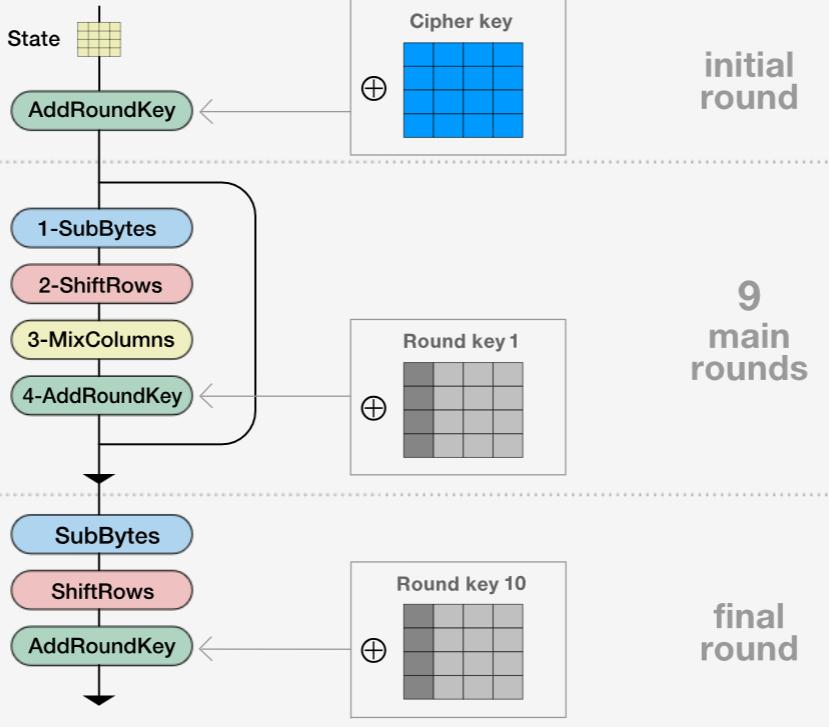
\includegraphics[width=0.5\textwidth]{img/aes-encryption-steps.jpeg}
    \caption{AES encryption steps. Source: Forma Estudio.\cite{aesanimation}.}
    \label{fig:aes-encryption-steps}
\end{figure}

The AES algorithm repeatedly applies four types of transformations as depicted in Figure \ref{fig:aes-encryption-steps}.
The figures in this section are from the Rijandael (AES) Animation made by Forma Estudio\cite{aesanimation}.
This animation explains the algorithm much better than my text, but here is my attempt.
The transformations are:
\begin{enumerate}
    \item \b{SubBytes}.
        Uses an S-BOX, i.e., a lookup table.
        Each cell is substituted (changed) with a value from the S-BOX.
        The value is chosen by taking the first byte from the cell to select the row, and taking the second byte to select the column.
    \item \b{ShiftRows}.
        Each row is rotated to the left with its index.
        The first row stays as-is, the second is rotated 1, the third is rotated 2, and the fourth is rotated 3.
    \item \b{MixColumns}.
        Each column is Galois-multiplied by a specific matrix.
        Galois-multiplication is a special type of multiplication, which gives results in the same set as its inputs.
        So this is yet another step to mix bytes up deterministically.
    \item \b{AddRoundKey}.
        The round key is XOR-ed with the current matrix (explained later).
\end{enumerate}

The \b{AddRoundKey} step mentions a round key.
Round key comes from the Key Scheduling part of the Rijandael algorithm.
The cipher key (input of the algorithm) is expanded into eleven partial keys: one for the initial round, nine for the main rounds, and one for the final round.
We can visualize the cipher key as a matrix yet again, and the round keys will be generated to its right, column by column (see: Figure \ref{fig:aes-key-schedul}).
Starting with the cipher key, up until all the columns are generated, the steps below are performed.
Note that, the steps marked with \b{*} are performed only if the column's position is a multiple of 4.
For the rest of the columns, only XOR applies.
\begin{enumerate}
    \item \b{RotWord*}.
         the column is rotated once, in upside direction.
    \item \b{SubBytes*}
        Same as for enctyption, using the same S-BOX.
    \item \b{XOR}
        The column is XOR-ed with the column 4 positions to the left.
    \item \b{Add*}
        The column is summed with a column from a specific constant matrix (Rcon) 
\end{enumerate}

\begin{figure}[htbp]
    \centering
    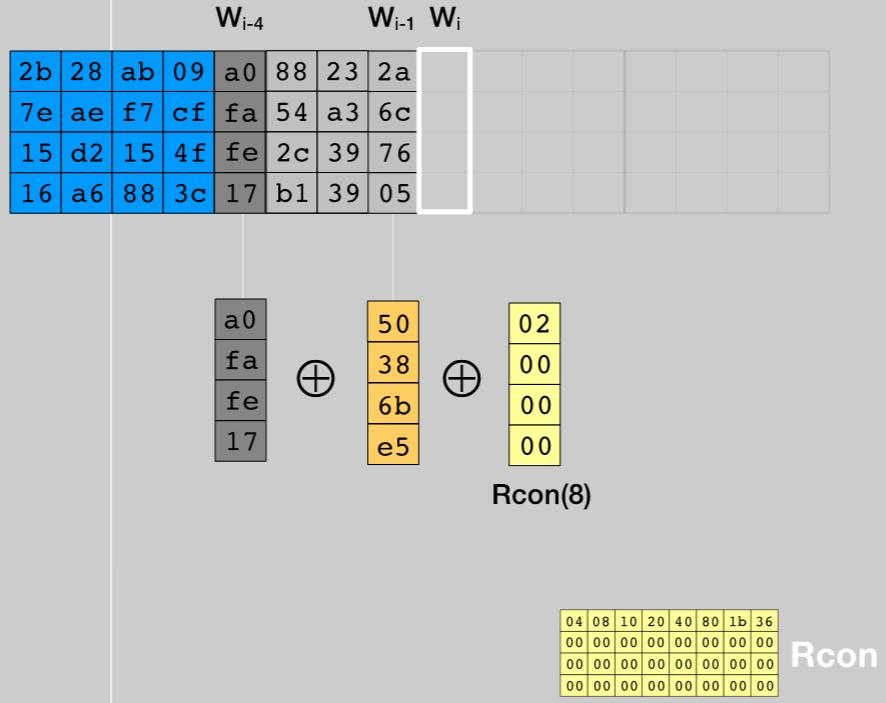
\includegraphics[width=0.5\textwidth]{img/aes-key-schedule.jpeg}
    \caption{AES Key Schedule. Source: Forma Estudio.\cite{aesanimation}.}
    \label{fig:aes-key-schedule}
\end{figure}

Now the amazing part is that encryption can be done the same way, but by reversing everything.
Instead of adding a matrix, we subtract it.
Instead of shifting to one direction, we shift to the opposite direction.
For substitution, we do the inverse substitution.
And Galois-multiplication has its inverse operation as well.
While some of these operations look complicated graphically, computers are really good at performing them, making encryption and decryption fast.
For its strong security, open-source nature and performance, AES is used in almost all cases when symmetric encryption is needed.



\section{Password-Based Key Derivation. PBKDF2} \label{lab:ch3-pbkdf2}



``In cryptography, a key derivation function (KDF) is a cryptographic algorithm that derives one or more secret keys from a secret value such as a master key, a password, or a passphrase using a pseudorandom function (which typically uses a cryptographic hash function or block cipher)''\footnote{\url{https://en.wikipedia.org/wiki/Key_derivation_function}}.
They are often used when keys need to be stretched or need to have a certain format.
A typical use case is applying password-based key derivation on a key before using it for AES.
If the key needs to be of a certain length, depending on the context, just padding it might break the security of the following algorithms, since it is predictable and not random.

Key derivation functions can not only enable random user input to be stretched to the required size, but it usually makes them harder to break as well.
These functions are intentionally slow, so that brute-force attacks and dictionary attacks are harder to be performed if inputs are being guessed.
If the key derivation is deliberately slow enough, it can be considered a hash function.
Such algorithms are, for example, crypt, bcrypt and scrypt.

The Password-Based Key Derivation Functions are examples of key derivation functions.
I used the word in plural since there are to major versions of it, PBKDF1 and PBKDF2.
``PBKDF1 applies a hash function, which shall be MD2, MD5 or SHA-1, to derive keys.
The length of the derived key is bounded by the length of the hash function output, which is 16 octets for MD2
   and MD5 and 20 octets for SHA-1.
(\dots)
PBKDF2 applies a pseudorandom function to derive keys. The length of the derived key is essentially unbounded.''\cite{pbkdf2}

I will focus on PBKDF2, as even the official publication describing them recommends it over PBKDF1.
The PBKDF2 algorithm has the following parameters:
\begin{itemize}
    \item $P$.
        A password, as an octet string (input).
        This is the password from which we want to derive a key.
        Usually user input, and we cannot rely on it being of a specific length or ``strength''.
    \item $S$.
        A salt, as an octet string (input).
        Just as usually, the salt has the purpose to bring randomness to the output.
        Even if the same password is provided, given that the salt is different, the hash will be different.
        This is a mechanism against brute-force and dictionary attacks.
    \item $c$.
        An iteration count, as a positive integer (input).
        It serves the purpose of increasing the cost of producing keys from a password.
        This way it also increases the difficulty of attack, making brute-forcing or building a dictionary take more time.
        The recommended minimum number of iterations is 1000.
    \item $dkLen$.
        The desired length of the derived key (input).
        This depends on what we want the key to use for later.
        But as principle, it can be different numbers, so the algorithm is capable of deriving different length keys.
    \item $PRF$
        The underlying pseudorandom function.
        Depending on which pseudorandom function is used, it might consume different length octets at a time.
        This length is refered to as $hLen$
\end{itemize}

First, the number of $hLen$-octet blocks of the derived key is calculated.
We simply take the total desired length and divide with the length taken at once, and ceil the result.
\begin{equation}
l = \left\lceil \frac{dkLen}{hLen} \right\rceil
\end{equation}

The number of leftover octets (for the last block) will be denoted with $r$.
\begin{equation}
r = dkLen - (l - 1) \times hLen
\end{equation}

Each block of the derived key ($T_i$) will come from the function $F$.
\begin{equation}
T_i = F(P, S, c, i) \quad \text{for } i = 1, 2, \dots, l
\end{equation}

And the function $F$ is the XOR of the first $c$ iterations.
\begin{equation}
F(P, S, c, i) = U_1 \oplus U_2 \oplus \dots \oplus U_c
\end{equation}

Where each iteration $U_i$ comes from applying $PRF$ on the password and different salts.
For the first iteration, the salt is $S$ concatenated with an encoded version of $i$ (the block index).
For the rest of the blocks, the salt is the result of the previous iteration.

\begin{align}
U_1 &= \operatorname{PRF}(P, S \parallel \operatorname{INT}(i)) \nonumber \\
U_2 &= \operatorname{PRF}(P, U_1) \nonumber \\
&\vdots \nonumber \\
U_c &= \operatorname{PRF}(P, U_{c-1})
\end{align}

After each block is calculated, they are concatenated.
From the last block we only take the first $r$ octets.
The result is the derived key, having the desired length.
\begin{equation}
DK = T_1 \parallel T_2 \parallel \dots \parallel T_l \langle 0 \dots r-1 \rangle
\end{equation}


\section{Hashing and Argon2} \label{lab:ch3-argon2}

``Hashing is a process that converts any input to a fixed-length, seemingly random output.''\footnote{\url{https://www.bitdefender.com/en-us/business/infozone/what-is-hashing}}.
For a function to be called hashing function, it has to fulfill certain criteria, aside of giving the same length output for any length input.
First of all, it has to be a one-way function.
Unlike for encryption, where we want the ciphertext to be decryptable, in case of hashing, it shall be impossible to convert the output of a hash function back to the input which it came from.
Hashes are compared between each other, or used as they are, but never reversed.

Then, it has to have good collision resistance.
Since we convert to a fixed size string, multiple inputs will give the same output, inevitably.
It is like parking infinite cars, in seemingly random order, into finite parking lots.
At one point, parking lots will fill up, and two cars will have the same lot.
This means that, if used for password storage and authentication, there is a mathematical chance that two passwords give the same hash, even with salting.
This would mean logging in with an incorrect password.
The catch is that for hash functions with good collision resistance, the chances are terribly low.
For example, for the MD5 algorithm, which was broken in 2004 (it was shown that it is not collision-resistant), the probability to have two passwords producing the same hash is $\frac{1.47}{10^{29}} = 0.0000000000000000000000000000147\%$.\footnote{\url{https://infosecscout.com/two-passwords-same-hash/}}.

The third criterion for a hash function to be considered usable is to be deterministic, not random.
That is why, in the last paragraph's analogy, I said ``seemingly random''.
The same input must give the same output all the time.
Otherwise, it would just be a random number generator, without the current practical use cases.

Hash functions are used for various purposes, out of which the most common are:
\begin{itemize}
    \item \b{Password storage.}
        Databases are often leaked, so storing the hash of a password instead clear text is the 101 of cybersecurity.
        In this case, it is extremely important to use a strong hashing algorithm, with proven collision resistance.
    \item \b{Fast look-up data structures.}
        Hash maps, for example, are often used where data has to be retrieved in \t{O(1)} time complexity.
        If we want to look for something, we compute its hash, which is the address it is supposed to be at.
        This way, we can instantly look up data.
        Collision resistance in this use-case is important for maintaining the speed advantage, not for security.
    \item \b{File signatures.}
        A hash function can take the contents of a whole file and convert it into a much shorter hash.
        This way, we get a unique value, a signature for each file (again, given that no collisions happen).
        We can easily check if a file changed, by looking at the previous and current signature.
        File signatures are also used for static malware analysis: we can take the hash of a program, feed it to a database like \url{https://www.virustotal.com}, and check if it is a reported malware.
\end{itemize}

Argon2\cite{argon2} is a password hashing algorithm, the winner of the Password Hashing Competition.
``PHC ran from 2013 to 2015 as an open competition—the same kind of process as NIST's AES and SHA-3 competitions, and the most effective way to develop a crypto standard.
We received 24 candidates, including many excellent designs, and selected one winner, Argon2, an algorithm designed by Alex Biryukov, Daniel Dinu, and Dmitry Khovratovich from University of Luxembourg.''\footnote{\url{https://www.password-hashing.net/}}.

The algorithm aims to maximize the cost of password cracking on Application-Specific Integrated Circuits (ASICs).
An ASIC is An ``integrated circuit designed for a specific customer, application, or market (\dots) interconnected, and simulated to provide the desired system functions and level of performance.'' \footnote{\url{https://www.analog.com/media/en/analog-dialogue/volume-24/number-3/articles/volume24-number3.pdf\#page=12}}.
In this context, it refers to hardware specialized for password cracking.
The advanced attackers who use such software often exploit parallelization (on GPUs, FPGAs, with more cores), they compute blocks ahead, they juggle with time-memory tradeoff (``the adversary can trade memory for time and do his job on fast hardware with low memory.''\cite{argon2}).

Argon2 takes all these aspects into account, and comes with a solution in two flavors: Argon2d and Argon2i.
Argon2d is faster and uses data-depending memory access, suitable for cryptocurrencies, for example.
Argon2i is slower and uses data-independent memory access, which is preferred for password hashing.
Data-dependent indexing takes into account the password when choosing the memory index to write to, this way making it impossible to prefetch and precompute missing data.
Some software, like Bitwarden, use Argon2id, which uses ``a combination of data-depending and data-independent memory accesses, which gives it some of Argon2i's resistance to side-channel cache timing attacks and much of Argon2d's resistance to GPU cracking attacks.''\footnote{\url{https://bitwarden.com/help/kdf-algorithms/}}

The mathematics behind Argon2 are out of scope for this document, but simply said, the algorithm consists of three steps.
First, memory initialization fills a defined memory size with pseudorandom values derived from the password, salt, and other parameters.
Then, the memory's contents are repeatedly combined with the password and the salt.
After all the iterations, the used memory is compressed into a fixed-size output (the hash).\footnote{\url{https://jumpcloud.com/it-index/what-is-argon2}}.
All this makes Argon2 an outstanding choice for password hashing, proven to be up-to-date with today's attackers.




\section{Full Disk Encryption and LUKS} \label{lab:ch3-luks}

Full disk encryption, as its name suggests, refers to encrypting every byte of a physical disk.
This mechanism is especially powerful since it provides a layer of security for the whole contents of a machine.
It also works for removable media.
With full disk encryption, an attacker's physical access does no longer mean compromised data.
With powerful encryption, brute-forcing decryption of a full disk takes so much time that it is virtually impossible.
``LUKS (Linux Unified Key Setup) is the standard disk encryption format for Linux, built on top of the dm-crypt kernel module.
It is the encryption layer used by default when you select “encrypt disk” during installation on Fedora, Ubuntu, Debian, and most other major distributions.''\footnote{\url{https://secure-os.org/articles/luks-encryption/}}.

It uses PBKDF2 to enhance weak user passwords and has a two level key hierarchy.\cite{luks}
This means that a master password is generated, which is not shared with the user, and the user's password is used to encrypt this master password, which is then stored in a slot.
There are several such slots (key material sections) in the LUKS header, meaning that multiple passwords can be used to decrypt the disk.
As a result, one can have a recovery key along the usual user password.

The LUKS header is the first few bytes of the disk which contains metadata needed for decryption (the algorithm, the KDF etc.).
It is a good idea to have a periodic backup of the LUKS header, since if this part of the memory is damaged, the whole disk becomes inaccessible.
It is a single point of failure, but there is no free meal.

LUKS2, the newer variant of LUKS, is a good option for encrypting disks and USB devices.
As with other cryptographic algorithms, there have been vulnerabilities in their implementation: in 2016, you could gain access by simply holding the enter button.\footnote{\url{https://hmarco.org/bugs/CVE-2016-4484/CVE-2016-4484_cryptsetup_initrd_shell.html}}.
But it is a good standard, and its open-source implementation is patched regularly.



\section{TPM} \label{lab:ch3-tpm}

``A Trusted Platform Module, also known as a TPM, is a cryptographic coprocessor that is present on most commercial PCs and servers'' \cite{tpmbook}.
This chip provides hardware-backed cryptographic primitives upon which software applications can build on.
Usually, when TPM is mentioned, it refers to the chip, which can come from different manufacturers, but must implement the specification defined by the Trusted Computing Group.

There are two main TPM specifications, one of them being TPM 1.2 (ISO/IEC 11889:2009) and the newer one being TPM 2.0 (ISO/IEC 11889:2015).\footnote{\url{https://en.wikipedia.org/wiki/Trusted_Platform_Module}}.
TPM 2.0 is not backward compatible with TPM 1.2.
While both specify similar features, TPM 2.0 is broader and is being pushed over its predecessor.
Since 2016, Microsoft has required all new PCs shipping with Windows 10 to include TPM 2.0 support.
When they released Windows 11 in 2021, the requirements contained TPM 2.0 support.
This caused major backlash, since many older PCs did not (and still do not) have this.
It is hard to find up-to-date exact statistics related to TPM 2.0 adoption rate, probably the least speculative number comes from Windows 11 adoption, as published by Microsoft (given that we trust them).
In March the 3rd, 2026, they stated that ``Windows 11 Dominates Desktop Share in 2026: ~73\% of Windows PCs''.\footnote{\url{https://windowsforum.com/windows-news.4/windows-11-dominates-desktop-share-in-2026-73-of-windows-pcs.403819/?spm=a2700.accio_bizSeo.0.0.180331dah3UXgl}}.
We can assume that most of these machines have TPM 2.0 (with some technical knowledge, or endorsement from Microsoft, this requirement can be bypassed).

A TPM is often refered to as a cryptographic coprocessor, a hardware security module (HSM) or a hardware root of trust (HToT).\cite{tpmpdf}
Its cryptographic functionalities include Random Number Generation (RNG), key generation, provides hashing functions and Hash Based Message Authentication Code (HMAC), as well as implementations for SHA-1, SHA-256, SHA-384, RSA,
ECC, AES, SM4 and XOR.
It also comes with volatile and non-volatile memory.
Volatile memory is used for authorization sessions and storing active keys.
Non-volatile memory has modules such as the Platform Configuration Registers (PCRs) and a limited Non-Volatile Random Access Memory (NVRAM).

The primary scope of TPM is to verify integrity during the boot process.
Its PCRs contain values which can be used ``to cryptographically record (measure) software state: both the software running on a platform and configuration data used by that software.''\cite{tpmbook}.
The state is hashed and the hash is used when booting to verify is the system was altered or not.

The NVRAM is used to store two types of data: data structures defined by the TPM architecture and unstructured data defined by a user.
An example use case mentioned by \cite{tpmbook} is storing a secret.
This memory is very limited in size, so it is not for storing large files.
Instead, the encryption key for a large file could be stored.

All in all, TPM 2.0 provides various hardware-backed cryptographic primitives, which could be used by the OS, but also by software running on a machine.
The TPM in itself is not a solution to all security problems neither.
Probably the biggest criticism of it came from the VeraCrypt developers, stating that ``The only thing that TPM is almost guaranteed to provide is a false sense of security.''\footnote{\url{https://veracrypt.io/en/FAQ.html}}.
Indeed, if the device is stolen, it is just a matter of time, technical skills and available resources before it is bypassed.
However, using its cryptographic primitives instead of software solutions is undoubtably stronger, with one catch - we have to trust the TPM manufacturer and vendor.


\chapter{Project Presentation} \label{lab:project-presentation}


\section{Proposed Framework} \label{lab:ch4-proposed-framework}

The goal of this Masters' thesis is to provide a generic framework for a TOTP application on a USB stick, as well as an implementation for it.
In this section, we will focus on the framework, i.e., the ideas and principles, rather than the technology used.
The presented framework could work on other devices as well, it is a generic flow of actions meant to be abstract.
At the same time, the framework's main goal is security, so it has to take into account all kinds of attacks and countermeasures for them.
With all that in mind, the framework focuses on minimizing the possibility of exploits, errors, deadlocks.

Simply put, a TOTP application generates TOTP codes (numbers) based on TOTP secrets (Base32 codes).
The application which requires TOTP (example: Gmail, Facebook, etc.) displays a QR code or an equivalent secret.
The user scans the QR code or introduces the secret manually into the TOTP application, which usually runs on a personal mobile device.
From that point on, the TOTP application stores that secret in a way or other, and keeps generating TOTP codes.

The framework aims to replace the mobile device with a USB stick.
This goal shall be achieved by fulfilling the following requirements:
\begin{enumerate}
    \item
        \b{Generate TOTP codes}.
        This is the main functional requirement of the framework.
        TOTP code generation is a standard algorithm and requires only the current time and the TOTP secret.
    \item
        \b{Store the secrets safely}.
        TOTP secrets are sensitive information.
        They shall be stored in a way which is secure and resistant to possible cyber-attacks.
    \item
        \b{Keep the 2FA aspect}:
        The framework treats the device on which the app runs as the possession factor of Two-Factor Authentication.
        Breaking this aspect would make the framework useless.
\end{enumerate}

Figure \ref{fig:flows} shows the two main flows of the proposed architecture.
It proposes the combination of three secrets: a password for encrypting the USB stick (\b{disk encryption password}), a password for unlocking the application and encrypting the secrets (\b{user password}), and optionally a TPM-provided secret which is combined with the user password for extra security (\b{TPM secret}).
Each of these will be detailed in the following sections.  
The following sections will go in depth on each aspect.

\begin{figure}[htbp]
    \centering
    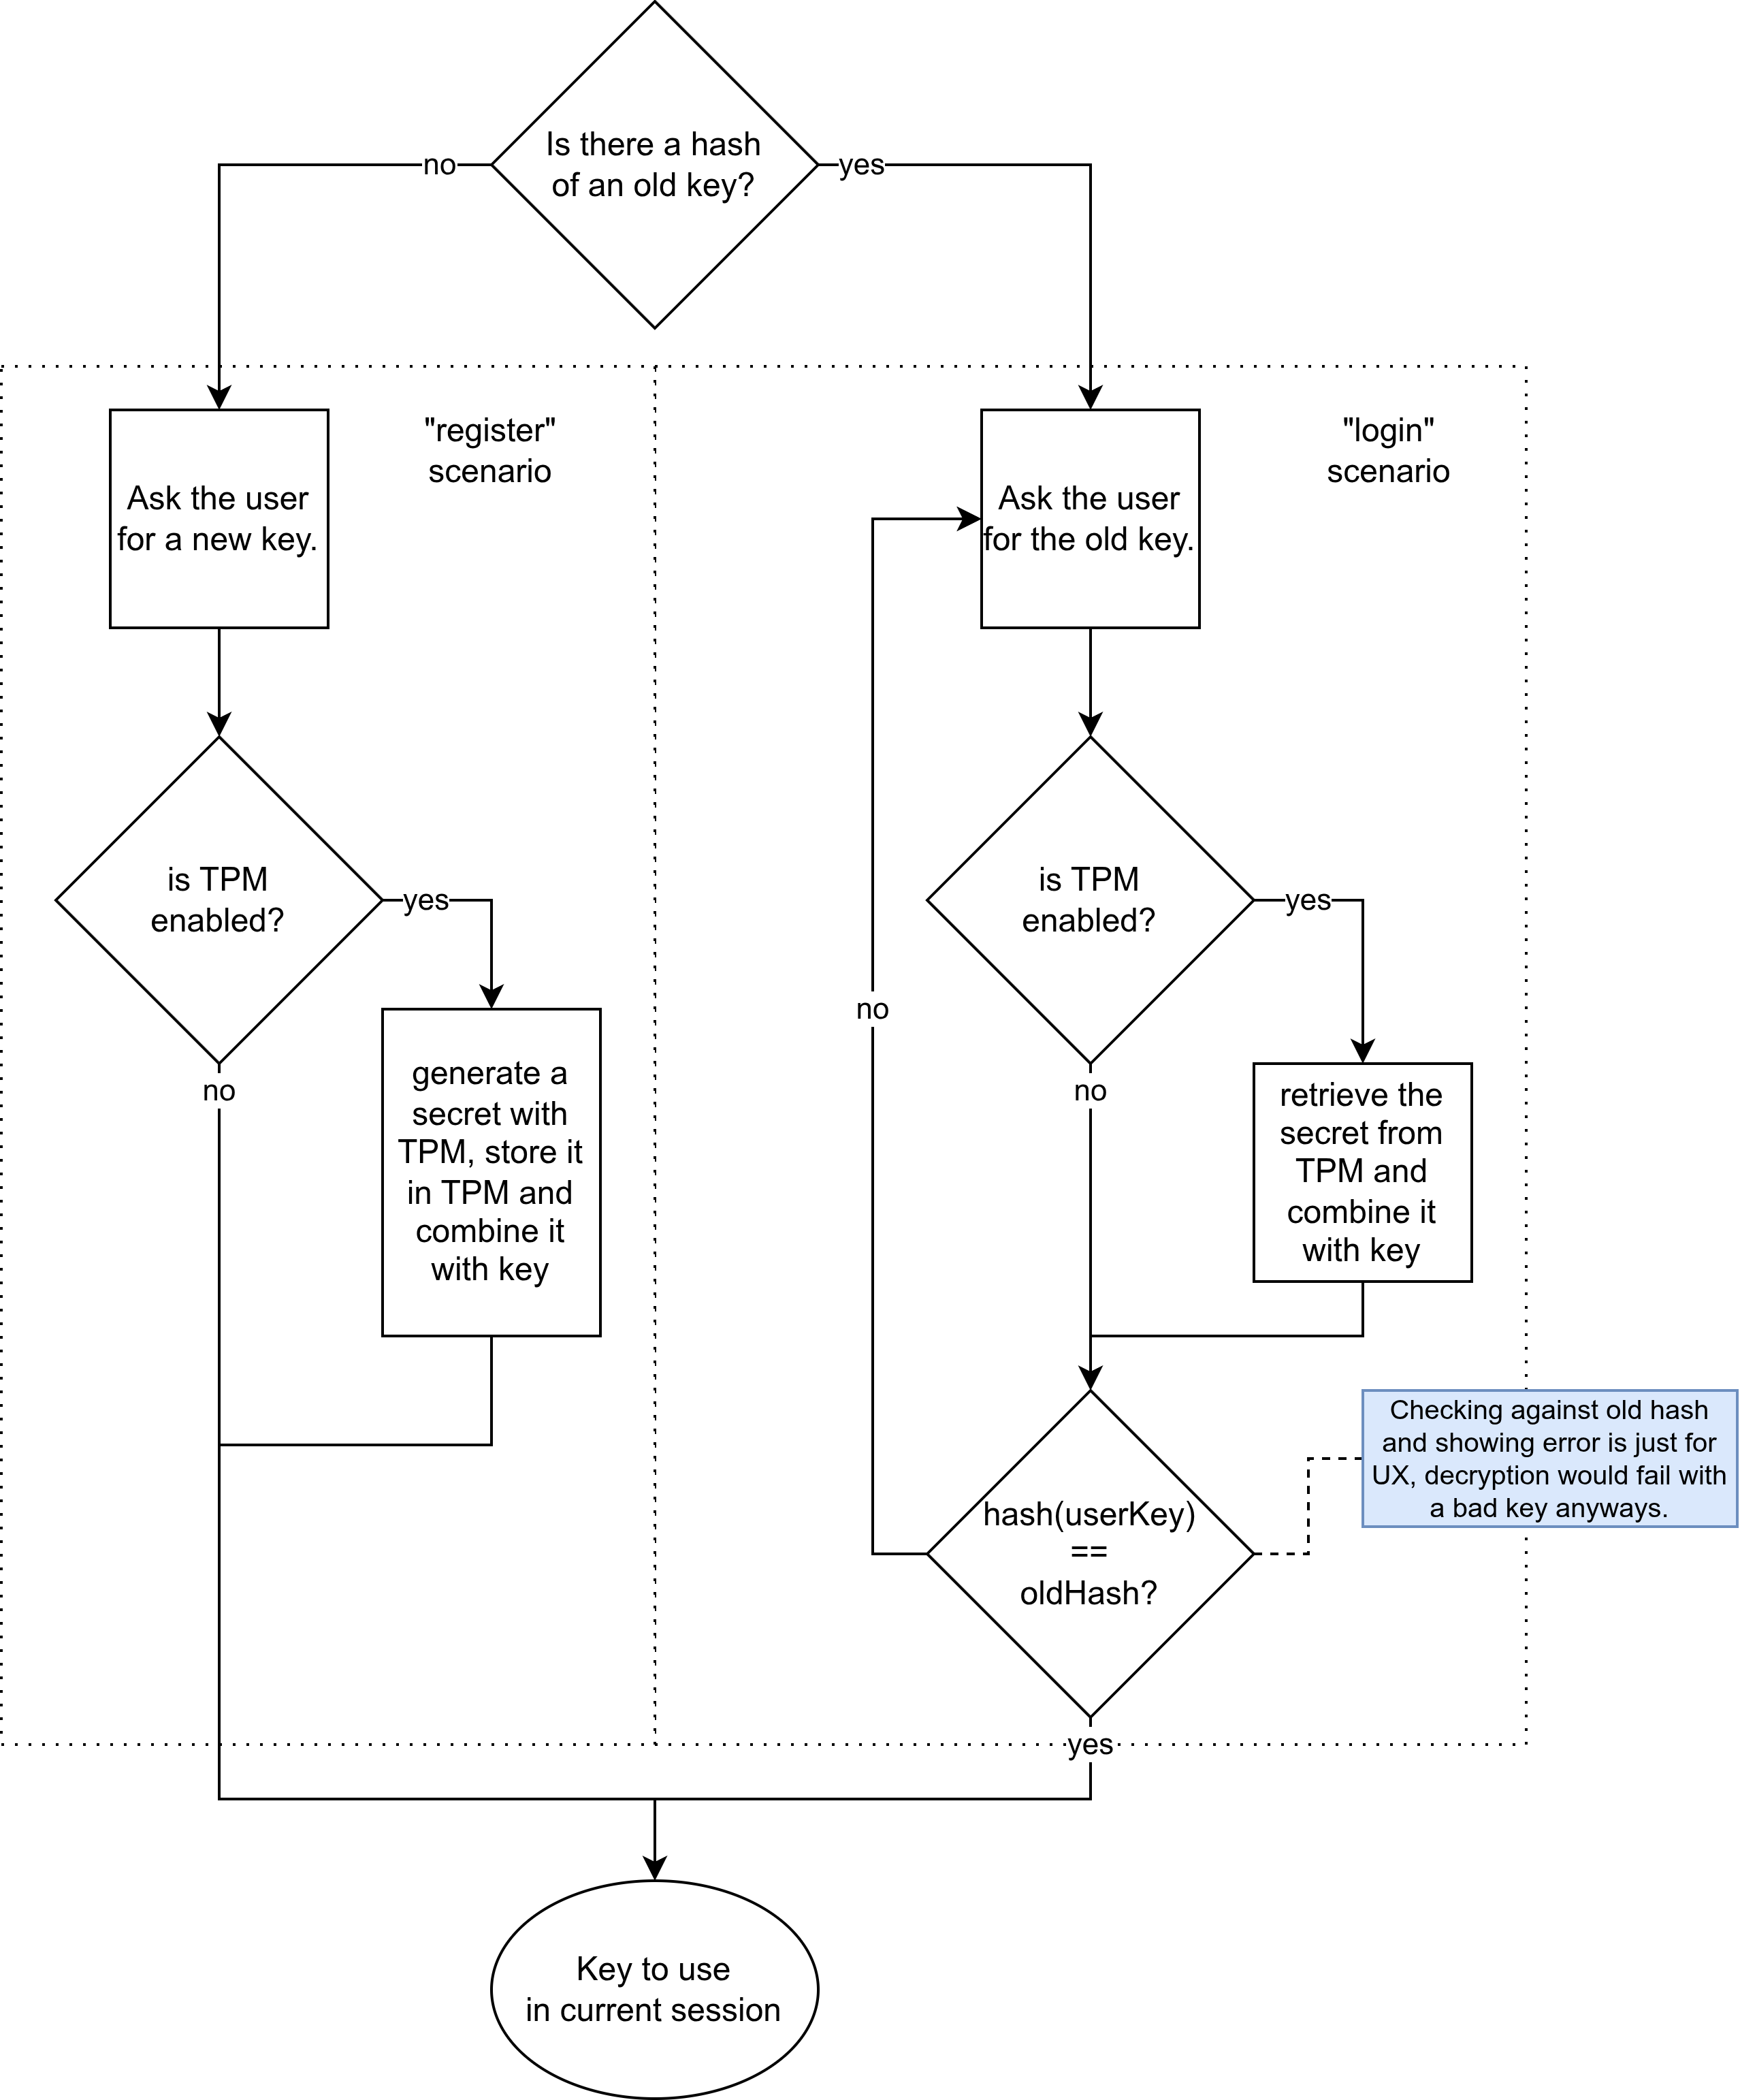
\includegraphics[width=\textwidth]{img/diagram-flows.png}
    \caption{The two main flows of the proposed framework.}
    \label{fig:flows}
\end{figure}

\subsection{Disk Encryption} \label{lab:ch4-disk-encryption}

The first line of defense is provided by the device on which the app resides: the USB itself shall be encrypted.
I will refer to the password used for the USB's encryption/ decryption as the \b{disk encryption password}.
Each operating system has specific USB formats and default disk encryption algorithms.
For Linux, Ext4 partition type encrypted with LUKS2 can be used (see: Section \ref{lab:ch3-luks}).
For Windows, W95 FAT32 partition type encrypted with BitLocker can be used.
The encryption of the device applies on its whole content.
This ensures that the stored secrets cannot be read without providing the disk encryption password.
Even if the running application saves passwords in plaintext, the USB encryption would encrypt it anyway.

The main issue of USB sticks (in our context) is that they are not read-only media.
Someone could steal the USB stick and copy its contents in less than a minute.
If the malicious actor puts the USB stick back to where he/she found it, the user would not even know.
The attacker could then brute-force breaking the USB without any time limitations.
Or even worse, if the attacker gets to know the disk encryption password, he/she can break in without having our media, using the copy.
Nevertheless, USB Encryption is a good first line of attack against not-so tech-savvy attackers.


\subsection{Storage Encryption} \label{lab:ch4-storage-encryption}

Aside of the password for the USB's encryption, the framework also requires a \b{user password}, for unlocking the application.
It is recommended for this password to be different from the password provided for the USB's encryption (see: Section \ref{lab:ch4-disk-encryption}), but a check for difference is out of scope.
So it is up to the user which user password it chooses, as long as it matches password complexity requirements.
The user password, aside of unlocking the application, is also used to encrypt the TOTP secrets the framework stores, in what we refer to as \b{storage}.

Of what use is another encryption on top of disk encryption?
You might ask, rightfully.
Well, disk encryption ensured data safety at rest, while the USB is locked, and storage encryption makes sure secrets are not stored in plaintext, even if the app is running and the USB is unlocked.
This protects against ``coffee-shop'' attacks: the user might leave their device unlocked and unsupervised.
In such cases, if the storage would be plaintext, an attacker could quickly read the secrets from their device.

Storage encryption is also a second layer of security on top of disk encryption.
While both could be brute-forced, if separate passwords are used for disk and storage encryption, the time required to do so increases.
While disk encryption algorithms might be more permissive regarding password complexity, and the framework has no control over it, the user password is required to be complex.
It is kind of a zero-trust scenario, where even if the user does not properly encrypt the disk it uses the framework on, the secrets are not leaked.

The user password is never stored.
Instead, the hash of the user password is stored inside a file, in what I refer to as the \b{hashed user password file}.
If the hashed user password file does not exist, the framework considers that no user password was provided beforehand.
The user is prompted to enter a new password.
This is the \b{register scenario}; although it is a one-user application, it is easier to refer to it with such standard naming.
If the hashed user password file exists at start, the framework considers that registering happened beforehand.
The user shall provide the old password, which is verified against the existing hash.
An incorrect password prevents the start of the flow, since the system has no knowledge about the password.
Without it, storage cannot be decrypted and secrets cannot be retrieved.


\subsection{Using TPM} \label{lab:ch4-using-tpm}

The read-write nature of a USB cannot be changed, and making a USB stick uncopiable is either impossible or out of scope.
The encryption with the help of the user password suffers the same vulnerability as the USB encryption, it is just another layer, but breakable in the same fashion.
Detecting if another TOTP Application is using the secret (for example, if the attacker stole the secret and introduced it into a TOTP application) is also out of scope.
However, the time required for brute-forcing can be made even bigger with the help of the Trusted Platform Module (TPM, see: Section \ref{lab:ch3-tpm}).

The framework proposes generating a random number with the TPM chip, further referred to as the \b{TPM secret}.
Since it is generated with dedicated hardware, it can be trusted (pun intended) to be truly random.
Its length shall be considerably large, for example, 16 bytes.
The TPM secret can then be combined with the user password in a cryptographically correct/ safe way, to produce what I refer to as the \b{key} or \b{key to use in current session}.
This shall be used for encrypting and decrypting the storage instead of using the user password directly.

One such combination method of the user password and the TPM secret is through the AES algorithm (see: Section \ref{lab:ch3-aes}).
The user password runs through PBKDF2 (see: Section \ref{lab:ch3-pbkdf2}), and the result is used as the initial secret of AES.
The TPM secret is long and random, perfect to be used as the salt of AES.
Brute-forcing this setup is unfeasible with current technologies.

The TPM secret has to be available on further sessions, since without it, the key cannot be derived.
It shall be stored in the TPM's NVRAM.
This is non-volatile memory, meaning that it will be present after reboot.
When needed, the NVRAM is queried for the TPM secret.
The TPM secret is not stored in any form (not even in a hashed version like the user password).

The main drawback of using TPM is the same as its main benefit: it ties the application to a specific machine.
If the user uses one machine all the time, this is not an issue.
If the user switches between multiple devices (which support USBs), he/she might consider not using TPM.
Also, setting up TPM is troublesome and requires technical abilities.
For these reasons, the framework marks TPM usage optional.
If TPM functionalities are disabled, a hardcoded salt is used instead of a TPM secret.


\section{Implementation} \label{lab:ch4-implementation}

The implementation of the proposed framework presented in Section \ref{lab:ch4-proposed-framework} is the application called \app{}.
To keep the code modular and maintainable, it follows the Model-View-Controller (MVC) architectural pattern, as depicted in Figure \ref{fig:high-level}.
The model consists of Python classes handling business logic and everything related, including storage.
The view is made with HTML, CSS and vanilla JavaScript.
The intermediaries between model and view lie in the controller package, which are Python classes as well.

\begin{figure}[htbp]
    \centering
    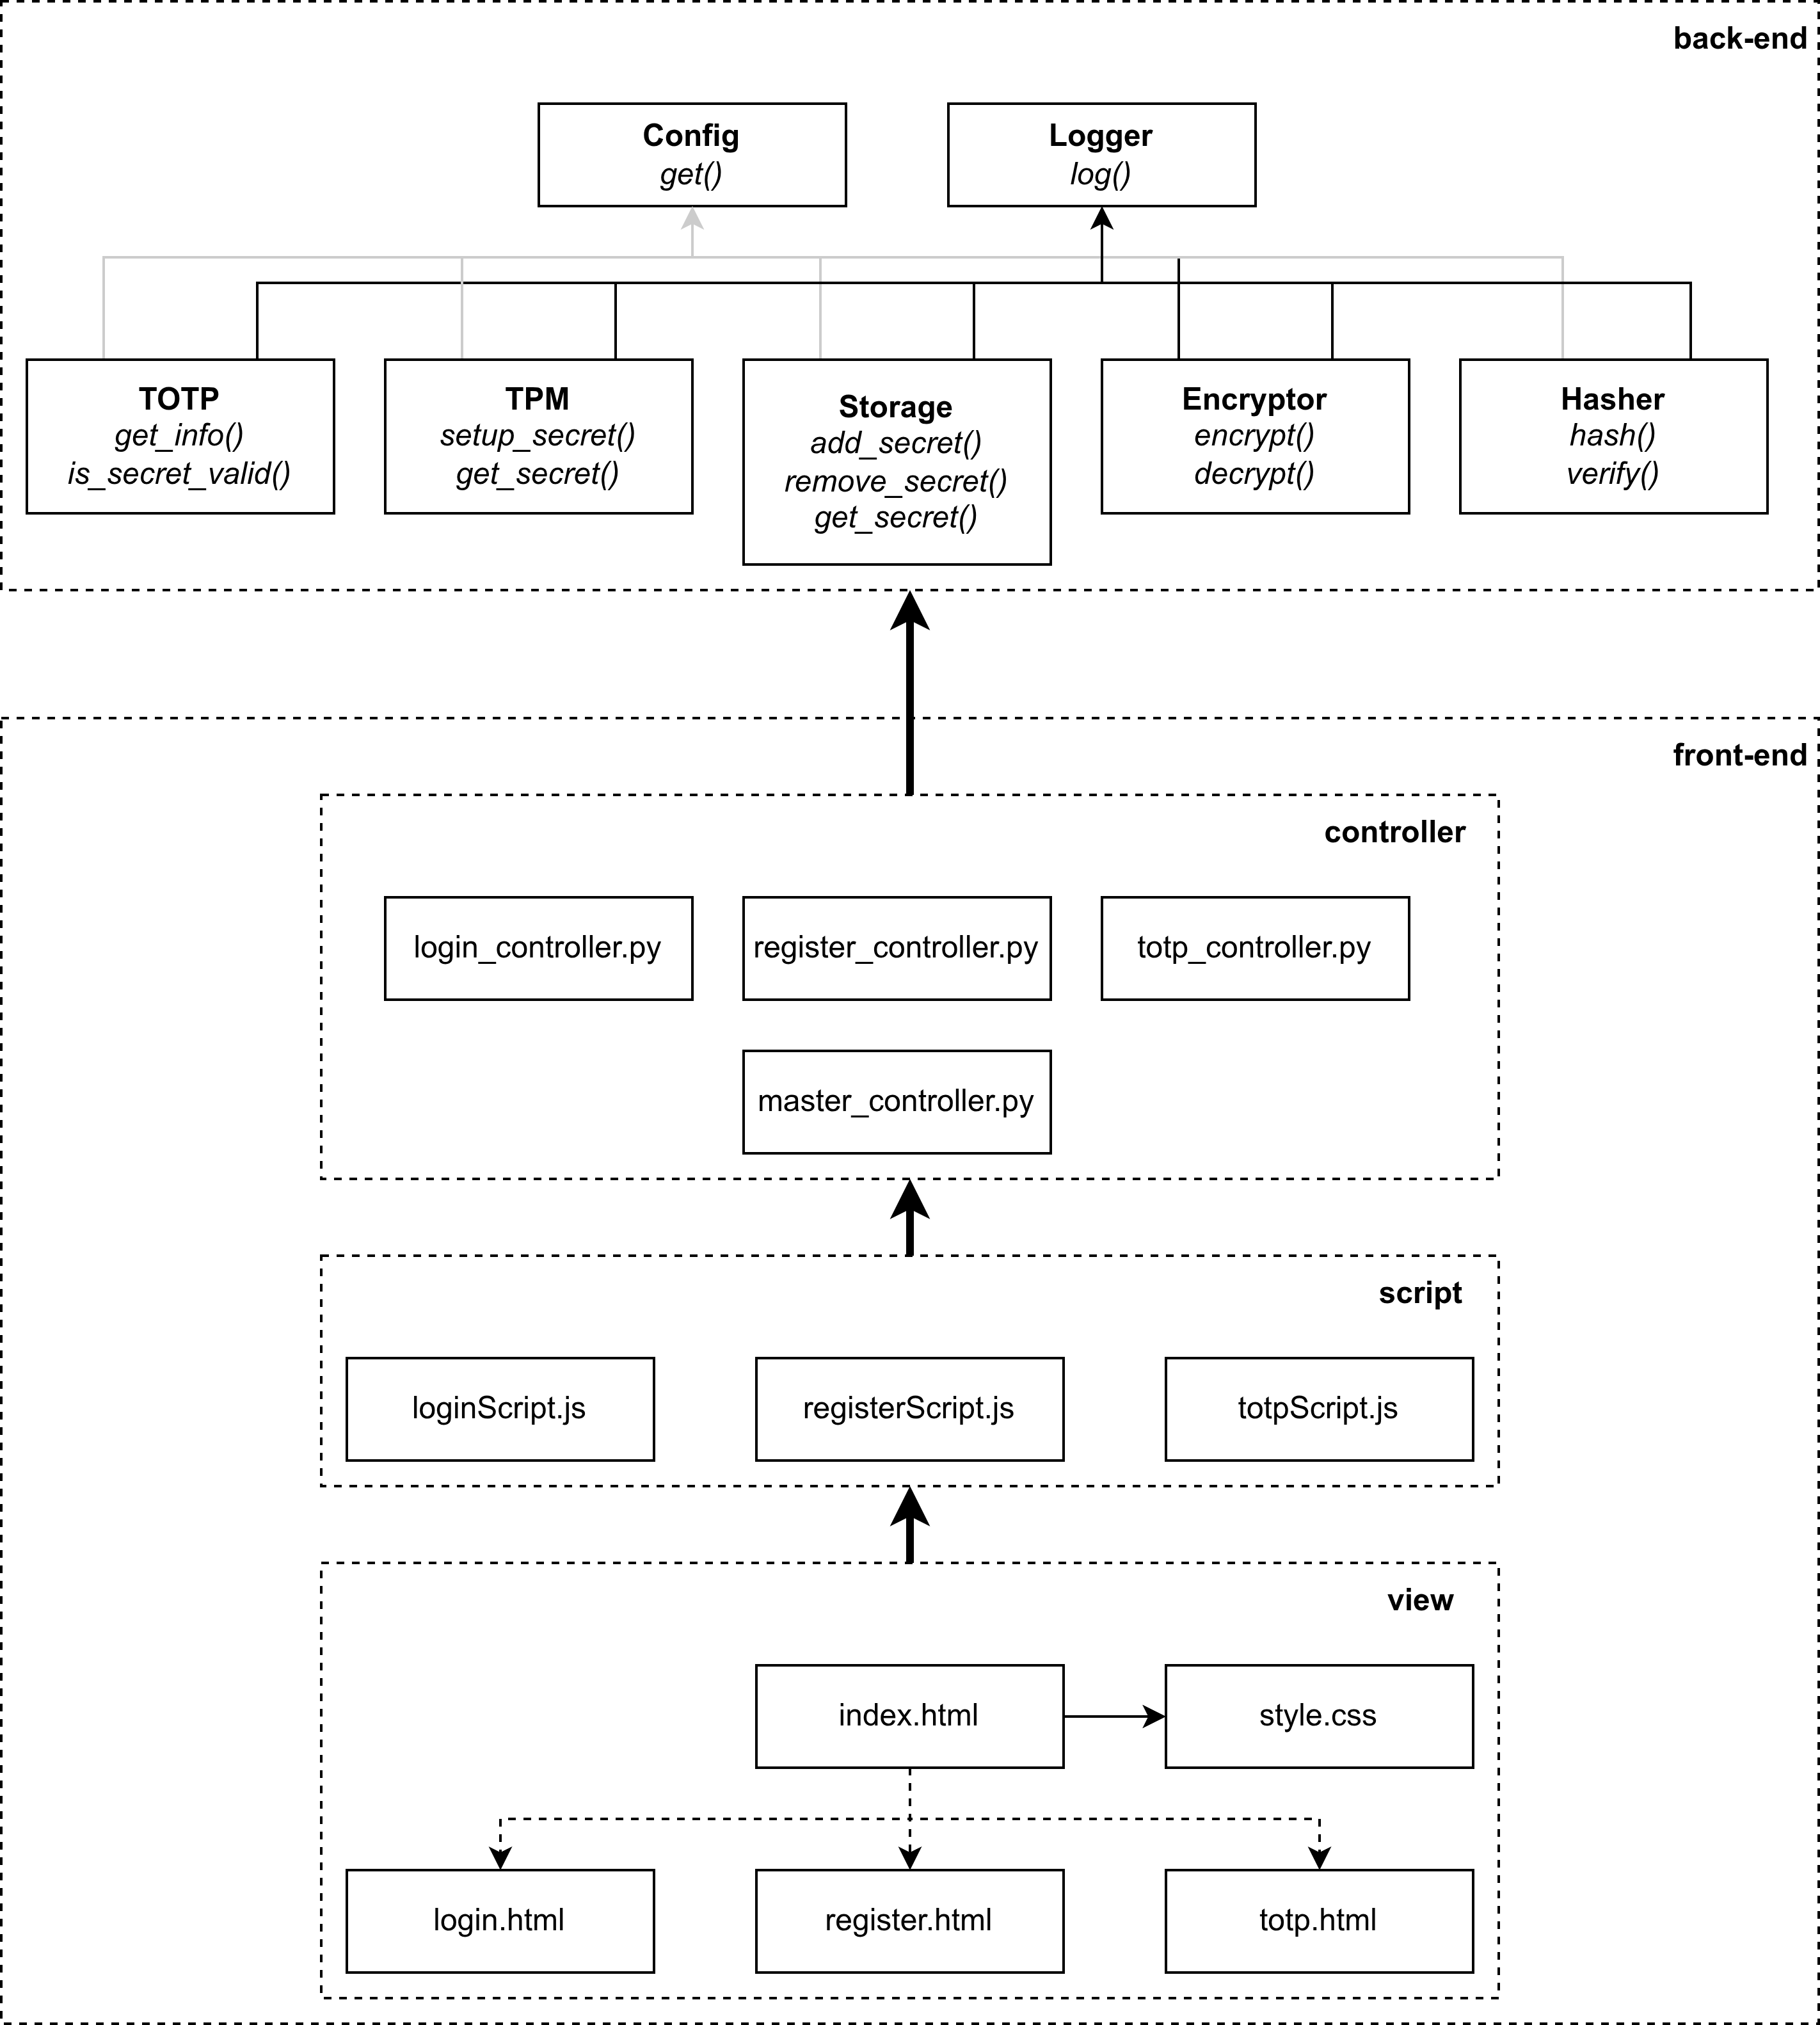
\includegraphics[width=\textwidth]{img/diagram-high-level.png}
    \caption{High-level diagram of \app{}.}
    \label{fig:high-level}
\end{figure}

\app{} uses the \t{pywebview} library to provide a desktop application GUI which is written in web technologies.
I chose to write HTML and CSS instead of using native GUI elements for a more uniform and cross-compatible experience.
I kept design simple, without going too heavy on JavaScript.
There are no JS libraries or frameworks included, since that would have a huge impact on the project size and performance.
Keep in mind that \app{} needs to run on a USB stick, so choosing lightweight solutions is a must.

Each of the packages will be described in detail in the following.
When thinking of flows, or when interpreting Figure \ref{fig:high-level}, keep in mind that everything is triggered by the actions of the user.
Flow always starts from view, where JS triggered by either the user interacting with HTML elements or by periodic method calls/ timers.
Then, the JS handler methods delegate to controller handler methods, which orchestrate the classes of model, calling business functionalities and tying them together.
The model classes are kept as independent as possible, and they are unit tested.

\subsection{Model} \label{lab:ch4-model}

As mentioned earlier, the back-end of the application is written in Python.
While it might sound like a weird choice for a security-first application, there are reasons for this decision.
First and foremost, Python provides a lot of libraries, making implementation easier.
Using standard implementations and not reinventing the wheel is usually the better approach for small teams.
This is even more true if we talk about cryptographic algorithms, like encryption and hashing.
\app{}'s backend contains plenty of these, so developing in Python enabled access to a lot of standard, popular, community-audited libraries.

Second of all, Python provides an easy way to manage dependencies.
When implementing \app{}, I also focused on making the developer experience easier.
The setup of a project is always a big pain in the butt; Python's package manager (\t{pip}) makes it bearable.
All the libraries are downloaded inside a virtual environment (\t{venv}), so they are isolated and do not mess with the system's packages.
The downloaded packages are then listed inside a \t{requirements.txt} file, so one can install all of them with a single command.

While Python isn't famous about its OOP capabilities, I chose an object-oriented approach.
For me and for most developers, it is simply a thing of habit to think of complex problems in terms of classes, objects, and interactions between objects.
It provides structure and a common language.
In \app{}, (almost) every Python file contains exactly one class, kind of like how Java enforces it.
Interfaces are implemented using \t{ABC} and \t{abstractmethod} from the \t{abc} library.
The overridden methods are marked with the annotation \t{override} from the \t{typing\_extensions} library.
These mechanisms do not cause runtime errors, but generate warnings in the right IDE, making it easier to catch bugs.

Similarly, the \t{typing} library is used for type hinting.
Python is duck-typed, meaning that for Python, if something quacks, it is a duck.
``The Python runtime does not enforce function and variable type annotations.''\footnote{\url{https://docs.python.org/3/library/typing.html}}, but the \t{typing} library provides runtime support for type hints.
The data type of method parameters and the return values of the methods can be specified. 
Mismatches will generate warnings.
Type hints also document intent: it is easier to understand what the method tries to achieve if you can picture the underlying data types.

The backend consists of several packages, which will be presented in the following sections.
Each package is self-contained, i.e., independent of the other.
As a result, they can be (and are) unit tested (see: Section \ref{ch5-theoretical-and-experimental-results}).
As a secondary side-effect, this isolation made it so that for most classes it made sense to use the Singleton pattern.
The singleton pattern ensures that there is just one instance of a given class at a time.


\subsubsection{Singletons, singletons everywhere.} \label{lab:ch4-singleton}

Since I wanted easily manageable classes, and probably since I am influenced by the fact that I worked with Java Beans for the last couple of months, all the classes of model follow the singleton pattern.
The main reason is philosophy: these classes encapsulate logic and state which shall be the same over the whole application.
Encryption, hashing, TOTP code generation etc. all work the same way, independently of where they will be called.
In some cases, static methods would have been enough, but for uniformity, and since static is not always an option, everything is a singleton class.

An example where singleton makes life easier than a pure static design: encryption.
While \app{} never stores the user password and the salt on disk, they are kept as class fields of singleton \t{Encryptor}.
Yes, this means the secret is stored in RAM, but so it is if it's just read for a split second.
Having it as class fields, we do not need to re-prompt the user at each encryption operation, nor to query the TPM for the secret each time.

There are two types of singletons in \app{}.
The classes with ``Manager'' in their name are simple singletons, for example, \t{LoggerManager}.
It contains a \t{instance} field.
If the constructor is called and \t{instance} is not None, it is returned instead of running a new initialization.
Else, \t{instance} is built up by filling its fields, running initialization logic and everything that happens in a constructor, as usual.
The seconds type of singletons define a facade for multiple classes.
For example, \t{TPM} is the TPM singleton: it has the usual singleton logic, but it also picks the right TPM class from a pool of multiple possibilities depending on the platform and the configs.
Each option implements \t{AbstractTPM}, which is the common interface.
This pattern is used where flexibility is desired: we want a singleton, but we have options for the specific class.


\subsubsection{Configurations and how \app{} is made parametrized.} \label{lab:ch4-config}

\app{} has certain parameters which can be changed from a JSON file, without changing source code.
The \t{config} package contains the \t{ConfigManager}, as well as one or two JSON files.
The \t{ConfigManager} is a singleton class, used by all of the classes of the model and controller.
It exposes a method, through which a JSON configuration file is parsed, and the config requested as a parameter is returned.
This way, the user of the application can change the behavior of \app{} without downloading a new release or changing the source code.

The name of the config file is hardcoded, and it is \t{config.json}.
It has multiple levels, as show in Listing \ref{lst:config-json}.
Developers also have the possibility to define a \t{config-local.json} file, which, if present, has priority over \t{config.json}.
The local config file shall be in \t{.gitignore} and used solely for local development.

\begin{lstlisting}[language=JSON, label={lst:config-json}, caption={An example configuration file.}]
{
  "logger": {
    "log_level": "DEBUG",
    "log_file_path": "log.txt"
  },
  "encryptor": {
    "type": "AES"
  },
  "hasher": {
    "type": "ARGON2"
  },
  "password": {
    "min_length": 15,
    "max_length": 100,
    "hash_file_path": "hash.txt"
  },
  "storage": {
    "storage_file_path": "storage.txt"
  },
  "pywebview": {
    "debug": false,
    "width": 450,
    "height": 800
  },
  "tpm": {
    "enabled": false,
    "virtual": {
      "fapi_profile": "P_RSA2048SHA256",
      "fapi_profile_url": "https://raw.githubusercontent.com/tpm2-software/tpm2-tss/3.2.0/dist/fapi-profiles/P_RSA2048SHA256.json",
      "enabled": false,
      "tpm_path": "/tmp/vtpm",
      "tpm_port": 2321,
      "tpm_ctrl_port": 2322,
      "tpm_start_wait_s": 1
    }
  }
}
\end{lstlisting}

The meaning of each parameter is the following:
\begin{itemize}
  \item \t{logger.log\_level}:
    The log level to use for the one and only logger.
    Everything higher or equal will be logged, everything lower will be ignored.
    Accepted options: \t{DEBUG}, \t{INFO}, \t{WARNING} \t{ERROR}.
  \item \t{{logger.log\_file\_path}}:
    The path of the log file.
    Logs are written to console but also to a log file, for audit, troubleshooting, and for cases there a console is not available.
  \item \t{encryptor.type}:
    The encryptor to use.
    As of v1, only \t{AES} is supported.
  \item \t{hasher.type}:
    The hasher to use.
    As of v1, only \t{ARGON2} is supported.
  \item \t{password.min\_length}:
    The minimum length required for user password, inclusive.
  \item \t{password.max\_length}:
    The maximum length accepted for user password, inclusive.
  \item \t{password.hash\_file\_path}:
    The path to the hashed user password file. 
  \item \t{storage.storage\_file\_path}:
    The path to the storage file.
  \item \t{pywebview.debug}:
    If set, pywebview's debug mode is enabled.
    Accepted options: \t{True}, \t{False}.
  \item \t{pywebview.width}:
    The width of the pywebview window.
  \item \t{pywebview.height}:
    The height of the pywebview window.
  \item \t{tpm.enabled}:
    If set, TPM functionalities are enabled.
    Accepted options: \t{True}, \t{False}.
  \item \t{tpm.virtual.fapi\_profile}:
    Which FAPI profile to use for the virtual TPM.
    Will be passed to \t{fapi-config.json}, and used as file name for the FAPI profile file.
    Must be in sync with parameter \t{tpm.virtual.fapi\_profile\_url}.
  \item \t{tpm.virtual.fapi\_profile\_url}:
    The URL from which the FAPI profile can be downloaded for the virtual TPM.
    Must be in sync with parameter \t{tpm.virtual.fapi\_profile}.
  \item \t{tpm.virtual.enabled}:
    If set, the software TPM is used instead the real TPM chip.
    Setup will run based on other \t{tpm.virtual} parameters.
    Accepted options: \t{True}, \t{False}.
  \item \t{tpm.virtual.tpm\_path}:
    Since TPMs on Linux are device nodes, this is the path to use for the virtual TPM.
  \item \t{tpm.virtual.tpm\_port}:
    The port to use for the virtual TPM.
  \item \t{tpm.virtual.tpm\_ctrl\_port}:
    The control port to use for the virtual TPM.
  \item \t{tpm\_start\_wait\_s}:
    The amount of seconds to wait before checking if the virtual TPM got successfully provisioned, after calling the provision function.
\end{itemize}


\subsubsection{How logging is done.}

Logging is done by the package \t{Logger}.
It contains the \t{LoggerManager} class, yet another singleton.
As its name suggests, the logger manager provides a logger instance.
It is the one and only way to print messages, the print statement and similar shall not be used.

The standard \t{logging} library is used.
The log level can be from config (see: Section \ref{lab:ch4-config}).
For simplicity, \app{} uses only four log levels.
It is important to select the right log level each time, otherwise important logs might get cluttered or not printed with certain configs.
From most severe to the least, these are:
\begin{enumerate}
    \item \b{Error}. For fatal issues, ones which break execution.
    \item \b{Warning}. For issues which should not be ignored, but do not crash the app.
    \item \b{Info}. For messages which are not issues, but things that might help in audit.
    \item \b{Debug}. The most low-level messages. These are useful only for development.
\end{enumerate}

While the logger is centralized, logging happens in two places: the console and the log file.
The same log lines are printed in both outputs, but the log file persists, meaning that new logs are appended to the old ones instead of starting a new file at each run.
This is helpful for debugging and provides a possibility to audit previous actions, for example, if someone else tried to log in.

The format of log lines is: date and time, severity level in a letter (E, W, I, D), the file and the line of the source, the logger, and the message itself.
Some log lines are shown on Figure \ref{fig:log-example}.
While there is only one logger instance, \t{pywebview}, the front-end library also logs its warnings and errors.
These are useful, so instead of throwing them out, they are ``propagated'' to \t{LoggerManager}'s instance.
This is why the logger is also printed in the log line: it can be either \t{[root]} or \t{[pywebview]}.

\begin{figure}[htbp]
    \centering
    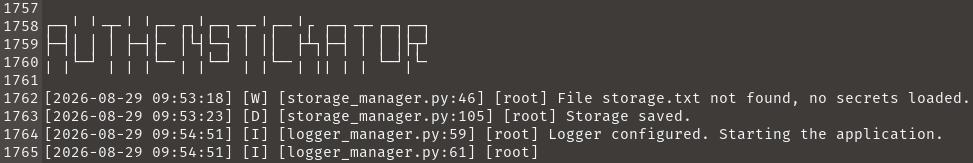
\includegraphics[width=\textwidth]{img/log-example.jpeg}
    \caption{Example log lines from the log file.}
    \label{fig:log-example}
\end{figure}

As a general rule, secrets and sensitive data shall never be logged.
Logging such information be the equivalent of a data leak.


\subsubsection{Generating TOTP codes.} \label{lab:ch4-totp}

Class \t{TOTPManager} is responsible for generating the TOTP codes, as well as other TOTP-related functionalities.
The \t{pyotp} library was used, which is straight-forward and provided every functionality I needed.
As a matter of fact, there are only two such functionalities: generating TOTP-related information and parsing TOTP URIs.

By \b{TOTP-related information}, I mean the current six-digit code, the next six-digit code, when the current code expires, and when the next code expires, as well as the interval.
The \b{interval} is the time for which one TOTP code is valid.
It is usually set to 30 seconds, as recommended by the authors of the TOTP algorithm.\cite{totp}
However, \app{} does not assume it is 30 seconds all the time, instead it deduces it from the secret.
Deducing the info from the secret is as simple as calling a constructor and then extracting its fields, although some mathematics had to be done.

Counterintuitively, I do not send to the frontend the seconds remaining.
This would be a huge overhead, just think about it: querying every second for every secret, just to get back the same redundant information roughly 58 times a minute.
Instead of querying each second, I could just automatically send each second, but again, this is a lot of redundancy, and it does get hacky.
Instead, what I chose to do, is to send the expiration times to frontend, and let the frontend calculate the remaining time.
Some kind of loop/ repetitive check is needed anyway, and a frontend timer is probably the best solution.
The frontend can then query for fresh information when the current code expires.

But what happens, if the querying takes longer than expected?
Or if the number of codes to query for is large, and they expire at the same time, causing an unexpected overhead?
Actually, the latter is rather expected, as almost all apps use the default TOTP parameters, and hence their codes all expire at the same moment (I have not seen any counter-examples yet).
Well, this is why I also send the next code.
It is trivial, and the TOTP algorithms allows us, to retrieve the next code.
In fact, any code could be computed, since the code is a function of the current time.
There are authenticator apps, like Proton Authenticator, which also show the next code.
So, the frontend has the current code and also the next one: when the current code expires, it can instantly \b{promote} the next code, i.e., make it current.
This results in a smooth transition.

\b{Parsing the TOTP URI} means extracting information from the URI which the apps usually show in QR form.
Yes, those fancy QR codes are nothing more than just a ``link'', which usually/hopefully follows the Key Uri Format specified by Google\footnote{\url{https://github.com/google/google-authenticator/wiki/Key-Uri-Format}}.
In the \t{TestTOTP} test class you can see some examples of such URIs, as different platforms provided to me:

\begin{enumerate}
  \item \url{otpauth://totp/totp@authenticationtest.com?secret=I65VU7K5ZQL7WB4E}
  \item \url{otpauth://totp/Google\%3Arolandtest123456\%40gmail.com?secret=refyopv7thgvsd5twr3marvdpqyugxls\&issuer=Google}
  \item \url{otpauth://totp/Microsoft:rolandtest123456@gmail.com?secret=G5HLROANXBF7335S\&issuer=Microsoft}
\end{enumerate}

The first one comes from the test site \url{https://authenticationtest.com/totpChallenge/}, which I used a lot throughout development.
It provides a hardcoded secret, both in plaintext and in QR form.
The QR, when parsed, resulted the URI shown with number 1.
Comparing it with the Key Uri Format examples, you can see that it contains the label \t{totp@authenticationtest.com}, and the secret \t{I65VU7K5ZQL7WB4E}.
It does not contain the issuer, although it is ``STRONGLY RECOMMENDED'' by Google, it is not required, hence we cannot assume that we get it all the time.
The second URI comes from a dummy Google account I made.
You can see that it used URL encoding\footnote{\url{https://www.calculator.net/url-encode-decode.html}}: \url{\%3A} $\rightarrow$ \t{:}, \url{\%40} $\rightarrow$ \t{@}.
The label also contains the issuer.
The third URI is from a dummy Microsoft account.
Similarly to number 2, this one also specifies an issuer, and the label already contains the issuer.

In \app{}, storage contains just two information: the secret and the name.
The name is combined as \t{ISSUER:LABEL}, if both available, or just the label, if it already contains the issuer, or just label, if issuer is not provided.


\subsubsection{Decoding QR images.}

Every mobile authenticator app provides the possibility to scan the QR code provided by the app which requires MFA.
But, a USB stick does not have a camera.
Initially, the only way to enter a TOTP secret into \app's database was to enter the secret manually, enter a name manually, and press enter.
But, what if the app only shows a QR, and does not give us the plaintext equivalent?
In that case, we could use an online tool to decode the QR image, but this would mean that we blindly trust a random website with handling out sensitive information.

As a solution, I integrated QR decoding functionality into \app{}.
It requires an image of the QR code, so a snip has to be saved beforehand.
\b{The user shall delete the screenshot after decoding it, or store it in a secure location.}
Otherwise, the secret could be exposed.
The app could delete the image after decoding, but it leaves it to the user; who am I to manipulate your files?
It would kind of break the isolation idea of \app{}, according to which the territory of \app{} is only the USB stick.

The QR code image is decoded using the \t{zxingcpp} library.
Initially, \t{pyzbar} was used, but it brought extra requirements for Windows packs, so I switched it to \t{zxingcpp}, which is newer and still maintained.
With the \t{pillow} library I opened the image, and with the \t{zxingcpp.read\_barcodes(image)} call I got the decoded text.
The text is a URI which is passed to TOTP for parsing (see: Section \ref{lab:ch4-totp}).
If there are no QR codes found in the image, I return None.
If there are multiple QR codes, the first one is processed, and a warning is logged.


\subsubsection{Hashing and checking against a previous hash.} \label{lab:ch4-hasher}

\app{} currently uses the Argon2 algorithm (see: Section \ref{lab:ch3-argon2}) in its \t{Argon2Hasher} class for hashing purposes.
The \t{argon2-cffi} library is used.
It provides a hashing and a verifying method.
It is worth noting that the same input creates different hashes, so verification is a library function call as well, not hashing and a simple equals operation.
The latter would not give correct results.


\subsubsection{Policies for the user password.}

The \t{PasswordManager} class implements the password policies for \app{}.
It is generally a good practice to extract password management into a separate class or module, to apply the same rules everywhere.
This is the only class which uses the user password hash file, no other classes shall read from or write to it, or modify it in any way.
The class exposes a method for checking if a previous password was provided, which does nothing more than check if the user password hash file exists.
This method determines upon startup if we go through the register or through the login scenario.

The password manager is also responsible for validating new passwords.
If they satisfy complexity requirements, it is said that they are ``acceptable''.
An acceptable password in \app{} has a length between a minimum and a maximum length specified by configs (see: Section \ref{lab:ch4-config}).
But, since \app{} takes security seriously, if the minimum length parameter is set to less than 15, it is switched to 15.
This is to follow the guidelines published by NIST SP 800-63B-4\footnote{\url{https://nvlpubs.nist.gov/nistpubs/SpecialPublications/NIST.SP.800-63B-4.pdf}}, Section 3.1.1, which says:
``Verifiers and CSPs SHALL require passwords that are used as a single-factor authentication mechanism to be a minimum of 15 characters in length.''

There is no special character requirement and such craziness.
We are well past the age where special characters provided any benefit.
Nowadays, they are rather an obstacle, in defining long a memorable passphrase.
The same NIST article, in its Appendix called Strength of Passwords, doubles down on this idea, saying that:
\begin{itemize}
  \item
    ``Password length is a primary factor in characterizing password strength''
  \item
    ``Research has shown that users respond in very predictable ways to the requirements imposed by composition rules.
    For example, a user who might have chosen “password” as their password would be relatively likely to choose “Password1” if required to include an uppercase letter and a number or “Password1!” if a symbol is also required.''
  \item
    ``Other mitigations (e.g., blocklists, secure hashed storage, machine-generated random passwords, rate limiting) are more effective at preventing modern brute-force attacks, so no additional password requirements are imposed.''
\end{itemize}

The password manager uses the hasher (see: Section \ref{lab:ch4-hasher}) to hash the user password before saving it to the user password hash file, and to verify the correctness of a provided user password, by reading the hash and verifying against it.
Setting a new password implicitly involves checking if the new password is acceptable.
There is also a hard limit of 100 maximum characters for the password, but this is just a sanity check, to avoid crazy users causing an overflow.


\subsubsection{TPM and the generation of the TPM secret.} \label{lab:ch4-tpm}

\app{} currently supports TPM functionalities only on Linux (see: Section \ref{lab:c6-further-improvements}).
Using the second singleton approach described in Section \ref{lab:ch4-singleton}, the \t{TPM} class chooses between \t{NoTPM}, \t{LinuxTPM} and \t{WinowsTPM}, where \t{WindowsTPM} contains identical implementation to \t{NoTPM}.
If TPM functionalities are disabled from configs (see: Section \ref{lab:ch4-config}), \t{NoTPM} is chosen.
Otherwise, the current platform dictates what to do.
\t{LinuxTPM} also provides support and setup for a virtual TPM, for development purposes.

As explained in \cite{pi3g_tpm_2025}, on Linux, TPM shows up as device nodes.
\t{/dev/tmp0} is the Hardware Interface, while \t{/dev/tpmtm0} is the Kernel Resource Manager.
Most applications use the Kernel Resource Manager, since through that entry the kernel handles context management and other low-level mechanisms.

TSS stands for Trusted Software Stack, and it is the software around the TPM chip.
It has a layered architecture, providing programmer-friendly API calls.
Its layers are specifications, and there are different implementations of it.
The four layers are:

\begin{enumerate}
    \item \textbf{FAPI}: Feature API. High-level, developer-friendly. No need to handle sessions and authorization.

    \item \textbf{ESAPI}: Enhanced System API. Wraps sessions and handles retries when TPM is busy.

    \item \textbf{SAPI}: System API. Low-level C interface implementing the tmp2.0 specifications.

    \item \textbf{TCTI}: TPM Command Transmission Interface. The Transport Layer, working with bytes.
\end{enumerate}

\app{} uses the \t{tpm2\_pytss} library and the FAPI layer.
FAPI was chosen since it is the most high-level, so the resulting code will be more generic.
Going lower in the TSS layers would mean more OS/ hardware specific code, and more chances to make errors.

When this layer is used, configurations are held in a file named \t{fapi-config.json}.
The default location is \t{/etc/tpm2-tss/fapi-config.json}, but it can be overwritten by setting the \t{TSS2\_FAPICONF} environment variable.
This file is generated automatically when you install or compile the libraries for FAPI provisioning, and it looks as shown in Listing \ref{default-fapi-config}.
\b{Provisioning} is an initialization step necessary to be performed before using FAPI.
The TPM, FAPI and the related files and configs are not well documented, so most of what I write here are the results of trial and error.

\begin{lstlisting}[language=json, label={default-fapi-config}, caption={The default FAPI configuration file, as on my system.}]
{
  "profile_name": "P_ECCP256SHA256",
  "profile_dir": "/etc/tpm2-tss/fapi-profiles/",
  "user_dir": "~/.local/share/tpm2-tss/user/keystore",
  "system_dir": "/var/lib/tpm2-tss/system/keystore",
  "tcti": "",
  "system_pcrs": [],
  "log_dir": "/var/run/tpm2-tss/eventlog/",
  "firmware_log_file": "/sys/kernel/security/tpm0/binary_bios_measurements",
  "ima_log_file": "/sys/kernel/security/ima/binary_runtime_measurements",
  "ek_cert_less": "yes"
}
\end{lstlisting}

Provisioning a real TPM might require authorization, or might have been done beforehand is there is other software using FAPI.
This is a tedious task which might differ from hardware to hardware, includes many edge cases and possible error sources.
I generated with the help of AI a setup script for provisioning, which worked on a fresh Ubuntu 22.04 installation, see Section \ref{lab:ch4-provisioning-the-tpm-on-linux}.
You can try it, or do it manually, but note that a provisioned FAPI is a prerequisite if you select non-virtualized TPM from configs.

For development, but strictly only for that, a virtual TPM is encouraged, which can be opted for through the configs.
By using a virtual TPM, you won't get locked out of the real TPM if you repeatedly violate authorization.
A virtual TPM can be wiped completely anytime, and a new instance can be started.
For the virtualization of the TPM, the \t{swtpm} Linux library is used.
The \t{LinuxTPM} class contains code for setup which should work out of the box, running each time if you selected virtualization.
It creates a custom \t{fapi-config.json}, as seen in Listing \ref{virtual-fapi-config}.

\begin{lstlisting}[language=json, label={virtual-fapi-config}, caption={The virtual FAPI configuration file, as on my system}]
{
    "profile_name": "P_RSA2048SHA256",
    "profile_dir": "/home/broland/.local/share/authenstickator/profile-dir",
    "user_dir": "/home/broland/.local/share/authenstickator/user-dir",
    "system_dir": "/home/broland/.local/share/authenstickator/system-dir",
    "tcti": "swtpm:port=2321",
    "system_pcrs": [],
    "log_dir": "/home/broland/.local/share/authenstickator",
    "ek_cert_less": "yes"
}
\end{lstlisting}

You can note the slight differences: there is a port defined, and a different profile is used.
The FAPI profile is downloaded from the internet, from the URL specified in the config file.
The profile's version shall match the version of the installed native \t{tpm2-tss/libtss2-fapi}.
This can be retrieved with the help of the command \t{apt policy libtss2-fapi1}.
Note that this is different from the \t{tpm2-pytss} version shown in \t{requirements.txt}.

If configuration, provisioning, and all the setup steps are done correctly and successfully, the actual usage of the TPM through FAPI reduces to just a few lines.
These high-level functions provide convenient wrappers for TPM functionalities.
The random number (TPM secret) is generated with \t{fapi.get\_random(16)}, where 16 means the secret will be of 16 bytes length.
This number is then saved to and later retrieved from the TPM's Non-Volatile Random Access Memory (NVRAM), using the \t{fapi.create\_nv}, \t{fapi.nv\_write} and \t{fapi.nv\_read}.
For each method, I used the same path, which basically defined the slot of NVRAM used, but abstracted, without going to index and byte level.
The existence of the TPM secret before generation is checked with \t{fapi.list("/")}, which gets a list of all FAPI object paths.
If the result contains our path, it means the secret was generated.

The FAPI method \t{create\_nv} is called with the flag \t{exists\_ok=True}, and \t{provision} (for the virtual TPM) is called with flag \t{is\_provisioned\_ok=True}.
Both of these, in the case of previous create/provisioning, write an error in the log files, but do not actually cause crash.
This is because \t{tpm2-pytss} is a wrapper for the \t{tpm2-tss} library written in C, and this is the best the wrapper's authors could come up, I guess.
This is a beauty flaw of the logs, but they do not mean actual errors.


\subsubsection{Encryption and decryption.} \label{lab:ch4-encryptor}

While the encryptor singleton allows the existence of multiple encryptors, currently only \t{AESEncryptor} is implemented.
As its name suggests, it uses the AES algorithm (see: Section \ref{lab:ch3-aes}).
The user password and the TPM secret is run through the PBKDF2 algorithm (see: Section \ref{lab:ch3-pbkdf2}).
This basically combines the user password, which could be of any length (between the limits imposed by the configs), and the TPM secret, which is used as salt, into a key of 32 bytes length.
The result can be used as a key for the AES algorithm.
AES is a symmetric algorithm, so the same key is used for encryption and decryption.

The libraries \t{Crypto.Cipher}, \t{Crypto.Hash} and \t{Crypto.Protocol.KDF} are used for \t{AES}, \t{SHA256} and \t{PBKDF2}, respectively.
For the PBKDF2 algorithm, I used 600000 iterations, with SHA256, as specified by the OWASP Password Storage Cheat Sheet\footnote{\url{https://cheatsheetseries.owasp.org/cheatsheets/Password_Storage_Cheat_Sheet.html\#pbkdf2}}.
This is a work factor, and having a high value means it is harder to brute-force, but slower for malign use as well (it is ``intentional slowness'').
So instead of balancing between security and usability with random trial and error, I consider that following trusted guidelines is a better option.

This AES library works with triplets of nonce, tag and ciphertext, i.e., the AES-EAX variant of the algorithm.
In practice, this means that at each encryption I create a new cipher using \t{AES.new}.
The ciphertext returned by the \t{AESEncryptor}'s \t{encrypt} method will then contain the nonce, concatenated with the tag and the actual ciphertext.
At decryption, this triplet is split.
A new cipher is created with the same key and the extracted nonce, and the tag is passed to \t{decrypt\_and\_verify} to ensure correctness.
This approach avoids the common pitfall of using the same nonce twice, which often turns such algorithms ``from gold-standard to broken'' (see \footnote{\url{https://www.trustedcalcs.com/en-us/guides/dev-tools/aes-gcm-encryption}} for an article which describes AES-GCM, which is another variant but at high level api point of view works the same way).

The \t{AESEncryptor} and its respective singleton class, \t{Encryptor}, went through multiple refactorings throughout development.
The final version does not set the key in the \t{\_\_init\_\_} method, but has a dedicated \t{set\_key} method.
This is because the user password can change: \app{} supports password reset.
In such cases, we want to change the key, but we do not want to swap out the singleton instance.
The \t{set\_key} solves this exact issue: the key (internal state) is changed, but the instance (the reference) remains the same, so the change is ``implicitly propagated'' throughout the code base.


\subsubsection{How the storage file is handled.}

The \t{StorageManager} class is the one responsible for handling storage.
Storage means the ``database'', which in practice is a single file, called the storage file.
The storage file's path can be defined as a config (see: Section \ref{lab:ch4-config}).
Storage manager uses the encryptor (see: Section \ref{lab:ch4-encryptor}) to decrypt the storage file upon initialization.
If encryption fails (either the key is wrong, although password checking should guard against this, or the file is broken, against which \app{} cannot protect), storage initialization is considered failed, and the \t{\_\_new\_\_} method returns None.
This has to be handled by the caller.

After successful decryption of the storage, the result is a JSON file which maps to a one-layer dict, where the key is the name (as described in Section \ref{lab:ch4-totp}), and the value is the TOTP secret.
The choice is intentional and would not work in reverse: the secret is provided by the user once, after which the UI only holds reference to the name, hence queries by name.
Keeping the secret in the UI would mean an information leak.
The fact that the underlying data structure is so simple makes saving trivial, symmetric to retrieval: the internal storage is dumped (\t{json.dumps}), the dump is encrypted, and the ciphertext is written to the file.

The class exposes methods for adding a secret, removing a secret, getting a secret.
There is also a ``get all secrets'' method, which shall be used at startup to load all the data.
These methods have straight-forward validations: an entry cannot be added if the name is already in use, an entry cannot be removed and/or retrieved if it does not exist.

Initially, I wrote the \t{StorageManager} to support the Context Manager Protocol, i.e., such that it can be used with Python's \t{with} syntax.
This meant that \t{StorageManager} was used inside a \t{with} block, and when execution got out of it in any form (the instructions were all executed or an exception happened), a cleanup function was called.
However, I found an even stronger and more robust solution: just save each time we modify storage.
This leaves no space (as in time window of intermediary instructions) for things to mess with storage.
If a secret is successfully added, the file is saved.
If a secret is successfully deleted, the file is saved.
This might sound like a huge overhead, but it is not: adding and removing secrets is not a frequent operation.
And, let's be real, how many TOTP secrets can a user have at most?






\subsection{View} \label{lab:ch4-view}

\subsection{Controller} \label{lab:ch4-controller}





\section{Development} \label{lab:ch4-development}

\app{} was developed on a relatively old laptop running Pop!\_OS 22.04 LTS.
For source control, just like every sane developer, I used Git.
The project is available as a public GitHub repository at \url{https://github.com/broland29/authenstickator}.
It has GPL-3.0 license, meaning it can be used freely as long as the product which uses is also open source.

The IDE used for development was PyCharm 2026.1.4.
The default Python formatter was used (Settings $\rightarrow$ Editor $\rightarrow$ Code Style $\rightarrow$ Scheme: Default), with a hard wrap at 100 columns.
100 characters is reasonable for Python code, for JS, HTML and CSS I did not set such limits.
I also set to format the code on each save (Settings $\rightarrow$ Actions on Save $\rightarrow$ tick Reformat code and Optimize imports).

The documentation was written in Latex, using Visual Studio Code 1.128.0 and the LaTeX Workshop extension.
For spell checking, the LTeX+ extension was used, which is completely offline.
The source code of the documentation is also under version control, available at \url{https://github.com/broland29/authenstickator-docs}, under the same license.
The starting point of the documentation was the template provided by the Technical University of Cluj-Napoca, available at \url{https://cs.utcluj.ro/studii-de-masterat/sesiunea-ii-septembrie-2026.html}.



\subsection{Dependency Management, Imports} \label{lab:ch4-dependency-management-imports}

For installing packages and keeping track of their versions, \t{pip} was used.
Some packages installed through \t{pip} also have OS-related dependencies, which will be discussed in later sections.
But, in principle, \t{pip} was the one and only source of packages.
Then, a \t{requirements.txt} file was generated using pip freeze.

\begin{lstlisting}[language=bash, label={lst:pip-freeze}, caption={Generating the requirements file.}]
pip freeze > requirements.txt
\end{lstlisting}

This file contains all the packages and their versions.
Even though \app{} was developed with cross-platform portability in mind, some functionalities, like the usage of TPM, required platform-specific packages.
These are also marked in the requirements file, like: \t{sys\_platform == "linux"}.
If, during development, new dependencies are added, or versions are updated, the command \ref{lst:pip-freeze} has to be run again.
But, be careful with updating packages: while I tried bringing everything to the latest version, there are some packages which simply do not work with newer versions, like \t{PyGObject}.

Dependencies are not installed directly on the whole system, but a virtual environment is used.
A virtual environment (\t{venv}) is used to isolate Python packages used for \app{} from other Python packages on the system.
This is standard dependency management, and ensures not just that \app{} works well, but that we don't break other apps.
Each developer creates its own virtual environment and these are not pushed to git (specified in \t{.gitignore}).

The application is run as a module (with the \t{-m} flag).
It is important to have every import start from the \t{src} folder.
Even if relative imports work in PyCharm (due to hacks PyCharm does in the background), not following this convention will have nasty side effects: running from the CLI with the usual command will simply not work.
The same convention has to be kept in tests also, since I hit unwanted side effects due to importing files differently in tests than in source code.
Make sure to set \t{authenstickator} as a Source Root (see: \footnote{\url{https://stackoverflow.com/questions/52949551/is-there-any-way-to-force-pycharm-to-always-use-absolute-imports}}).



\subsection{Setup and Packing}
\app{} is meant to run on a USB Stick, on machines which possibly do not even have Python.
One such release candidate is made with the help of PyInstaller.
``PyInstaller bundles a Python application and all its dependencies into a single package.
The user can run the packaged app without installing a Python interpreter or any modules. (\dots{})
However, it is not a cross-compiler; to make a Windows app you run PyInstaller on Windows, and to make a Linux app you run it on Linux, etc.
''\footnote{\cite{https://pyinstaller.org/en/stable/}}

Packing commands also differ on Linux and on Windows.
For example, executables' icons are treated differently.
For Linux, a lot of desktop environments (GNOME, KDE, Xfce) use \t{.desktop} files to tie the icon to the application launcher.
Since these files need absolute paths, and the app is run on a USB stick, I simply gave up on giving an icon for the Linux version.
Power users are welcome to create their own \t{.desktop} files.
The icon is available in the source code as \t{logo.png}.
For Windows, a \t{.ico} file is required, which can be specified as an argument for the PyInstaller, and will be embedded inside the \t{exe} file.


\subsection{Setup on Linux}\label{lab:ch4-setup-on-linux}

The following setup was tested on Ubuntu 22.04 LTS.
It might work on other Debian-based systems as well, but there is no guarantee.
Development was done with Python 3.10.12, which came with the OS installation.

Some Python dependencies from \t{requirements.txt} require specific Linux packages to work.
These include: a build compiler, the TPM2 development headers and build tools, some FAPI requirements (TPM-related), and some \t{PyGObject} requirements (\t{pywebview}/ UI related).
For development, to avoid TPM lockout, a software TPM, \t{swtpm} is recommended, which also needs installation.
Be careful with the \t{apt install} command: if you accidentally leave spaces after the line-breaking backslashes, it won't work.
After it finishes, the project is cloned, a virtual environment is created, and requirements are installed inside.

\begin{lstlisting}[language=bash, label={lst:linux-setup}, caption={Setup commands for Linux.}]
sudo apt-get update

sudo apt install -y git \
  python3.10 python3.10-venv \
  build-essential \
  libtss2-dev pkg-config python3-dev \
  libssl-dev libjson-c-dev libcurl4-openssl-dev \
  libgirepository1.0-dev libcairo2-dev libglib2.0-dev gobject-introspection \
  swtpm

git clone https://github.com/broland29/authenstickator.git
cd authenstickator

python3 -m venv venv
source venv/bin/activate

pip install -r requirements.txt
\end{lstlisting}


Once the scripts from \ref{lst:linux-setup} all finished, you can start the app.
Always activate the virtual environment before running.
\begin{lstlisting}[language=bash, label={lst:linux-run-app}, caption={Running the app on Linux.}]
python3 -m src.main
\end{lstlisting}

To ensure that the app is properly working, you can run the unit tests:
\begin{lstlisting}[language=bash, label={lst:linux-run-tests}, caption={Running the tests on Linux.}]
python -m pytest
\end{lstlisting}



\subsection{Provisioning the TPM on Linux} \label{lab:ch4-provisioning-the-tpm-on-linux}

If you want to use \app{} with the TPM feature enabled, you need to provision the TPM.
If not, you can skip this section.

\subsubsection{Real TPM}
Check if you actually have a TPM chip.
\begin{lstlisting}[language=bash, label={lst:tpm-check}, caption={Check if you have a TPM.}]
sudo dmesg | grep -i tpm
ls -l /dev/tpm0 /dev/tpmrm0
\end{lstlisting}

Having a physical TPM chip (or a simulated one, if you are on a VM) is a hard requirement for TPM functionalities.
See Figure \ref{fig:tpm-check} for example outputs if you have it or not.
\begin{figure}[htbp]
    \centering
    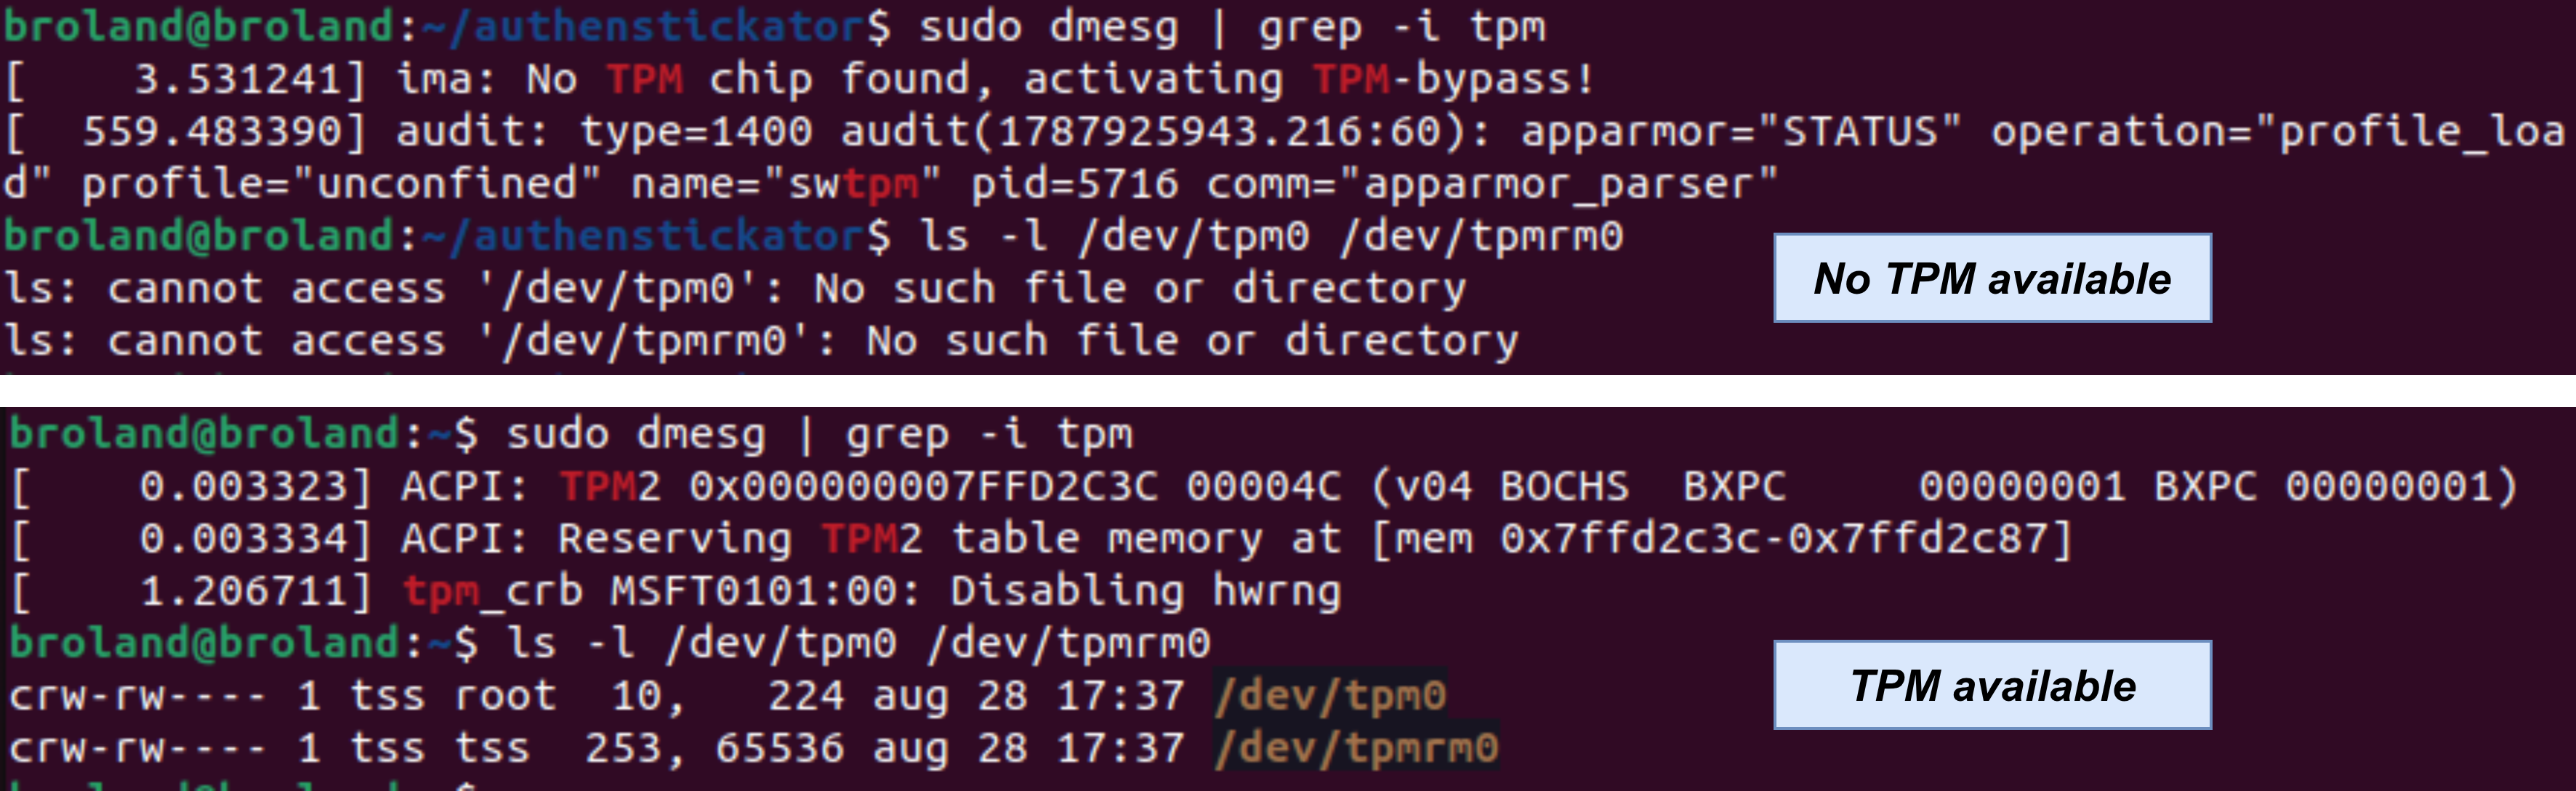
\includegraphics[width=\textwidth]{img/tpm-check.png}
    \caption{Check if you have a TPM.}
    \label{fig:tpm-check}
\end{figure}

For provisioning, you will need to run the \t{tss2\_provision} command of package \t{tpm2-tools}.
You can try getting it through \t{apt}, but it did not work for me.
\begin{lstlisting}[language=bash]
sudo apt install -y tpm2-tools
sudo -u tss tss2_provision
\end{lstlisting}

If you get a command not found error, welcome to the club.
The alternative is to compile \t{tpm2-tools} from source.
This package requires the \t{tpm2-tss} package, which also needs to be compiled from source with a compatible version.
I generated a script with Gemini, found in the repo under \t{script/setup\_fapi.sh}.
It can be run as shown in Listing \ref{lst:setup-fapi}.
This script:
\begin{enumerate}
  \item Installs dependencies for \t{tpm2-tss} and \t{tpm2-tools}.
  \item Adds your user to the \t{tss} group. You will run \app{} as your user, and interacting with TPM requires membership of this group.
  \item Compiles \t{tpm2-tss v4.1.3}.
  \item Compiles \t{tpm2-tools v5.6}.
  \item Removes some FAPI profiles which were too modern for Ubuntu 22.04 and adds \t{ek\_cert\_less = "yes"} to the automatically generated \t{fapi-config.json}.
  \item Creates the directories necessary for provisioning, and provisions.
  \item Generates a random number to see if TPM responds (although this does not require provisioning).
\end{enumerate}

\begin{lstlisting}[language=bash, label={lst:setup-fapi}, caption={Running the FAPI setup script.}]
chmod +x ./script/setup_fapi.sh
sudo ./script/setup_fapi.sh
\end{lstlisting}

If you mess with the TPM too much, it will lock you out.
TPM is protecting itself against dictionary attacks (DA), by disallowing further commands for a period of time.
This time period can be pretty long (don't ask me why I have this knowledge).
One possible solution to get out of the lockout is a command I found in a thread from Ubuntu\footnote{\url{https://documentation.ubuntu.com/core/how-to-guides/manage-ubuntu-core/troubleshooting/}}, shown in Listing \ref{lst:tpm-lockout}.
The file it modifies contained the value 0 when I was locked out, so it is probably a reversed violation counter.
Without a system reboot, the change has no effect.

\begin{lstlisting}[language=bash, label={lst:tpm-lockout}, caption={Getting out of TPM's Lockout Mode.}]
echo 5 | sudo tee /sys/class/tpm/tpm0/ppi/request
reboot
\end{lstlisting}

Also, if you get provisioning errors saying that TPM was already set up, you might want to try deleting previous keystores (see: Listing \ref{lst:wiping-keystores}).
These affect only FAPI, not the whole TPM (I have disk encryption which uses TPM, but this command did not break it).
If other software on your PC uses FAPI, you might want to look for a more graceful solution.

\begin{lstlisting}[language=bash, label={lst:wiping-keystores}, caption={Wiping previous keystores.}]
sudo rm -r /var/lib/tpm2-tss/system/keystore/
rm -r ~/.local/share/tpm2-tss/user/keystore/
\end{lstlisting}

The default \t{fapi\_config} is generated while compiling tpm2-tss and tpm2-tools.
It can be found at the path \t{/etc/tpm2-tss/fapi-config.json}.
After the script's modifications, it might look like on Listing \ref{lst:default-fapi-config}.
\begin{lstlisting}[language=json, label={lst:default-fapi-config}, caption={The default \t{fapi-config.json}, after the script's modifications.}]
{
  "profile_name": "P_ECCP256SHA256",
  "profile_dir": "/etc/tpm2-tss/fapi-profiles/",
  "user_dir": "~/.local/share/tpm2-tss/user/keystore",
  "system_dir": "/var/lib/tpm2-tss/system/keystore",
  "tcti": "",
  "system_pcrs": [],
  "log_dir": "/var/run/tpm2-tss/eventlog/",
  "firmware_log_file": "/sys/kernel/security/tpm0/binary_bios_measurements",
  "ima_log_file": "/sys/kernel/security/ima/binary_runtime_measurements",
  "ek_cert_less": "yes"
}
\end{lstlisting}

\subsubsection{Virtual TPM}

To run with a virtual TPM, change the configs to enable it (see: Section \ref{lab:ch4-config}).
It should work out of the box.
But if you have to troubleshoot, you can check manually if \t{swtpm} is running using \t{netcat} (see: Listing \ref{lst:check-swtpm}).
While \app{} runs, the command should output something like ``Connection to localhost (127.0.0.1) 2322 port [tcp/*] succeeded!''.
Run it multiple times, the first one might fail.
Make sure the ports match the ones in configs.
\begin{lstlisting}[language=bash, label={lst:check-swtpm}, caption={Checking if the virtual TPM is running.}]
nc -zv localhost 2322
\end{lstlisting}

If \t{swtpm} locks you out and/or you want to start fresh, you can kill its process and delete its folder.
\begin{lstlisting}[language=bash]
pkill swtpm | rm -r /tmp/vtpm
\end{lstlisting}

Then, you can re-launch the app, or run the commands from \t{linux\_tpm.py} manually.



\subsection{Packing on Linux}

To pack \app{}, after a successful setup (see: Section \ref{lab:ch4-setup-on-linux}), run the Linux packing script, as in Listing \ref{lst:packing-linux}.
If you ran it previously, it will prompt you if you want to overwrite existing data, and you need to press Y.
The flags specified in \t{pack-linux.sh} add a name to the packed executable, add non-Python files which \t{pyinstaller} would not include by default, ensure paths start from root, and specify the output directory.
Builds are generated in the temporary folder, so they will be wiped at reboot; you can change this if you wish.

\begin{lstlisting}[language=bash, label={lst:packing-linux}, caption={Running the packing script for Linux.}]
source venv/bin/activate
pip install pyinstaller
./script/pack-linux.sh
\end{lstlisting}

If you want to create a release/archive, navigate to the previous command's output (by default \t{/tmp/authenstickator/dist}) and pack it using \t{tar}.
See Listing \ref{lst:archive-linux} for an example of packing for an Ubuntu release, and later extracting.
If you did this on a VM and want to get the archive to your host machine, on the VM, you can get your IP (\t{YOUR-VM-IP}) using \t{ip a}, then start a local HTTP server with Python using \t{python3 -m http.server 8000}.
After that, you can connect through your host's browser through \url{http://YOUR-VM-IP:8000/}.

\begin{lstlisting}[label={lst:archive-linux}, caption={Create archive and extract on Linux.}]
tar -czvf Authenstickator-v1.0.0-Ubuntu-22.04.5-LTS.tar.gz Authenstickator/
tar -xzvf Authenstickator-v1.0.0-Ubuntu-22.04.5-LTS.tar.gz
\end{lstlisting}



\subsection{Setup on Windows} \label{lab:ch4-setup-on-windows}

The following setup was tested on Microsoft Windows Version 10.0.19045.6466.
It might work on other Windows systems as well, but there is no guarantee.

Although development was done with Python 3.10.12, for Windows, this version does not have a binary release.
Instead, you can get 3.10.11 from \url{https://www.python.org/downloads/release/python-31011/}.
When running the installer, tick the option to add to path and to disable path length limit.
You will also need Git, you can get it from \url{https://git-scm.com/install/windows}.
After having Python and Git, run the commands from Listing \ref{lst:windows-setup}.
Command \t{where python} shall output as first entry \t{$\backslash$venv$\backslash$Scripts$\backslash$python.exe}; if not, try activating again/ in a new terminal (it happened to me).

\begin{lstlisting}[language=bash, label={lst:windows-setup}, caption={Setup commands for Windows.}]
git clone https://github.com/broland29/authenstickator.git
cd authenstickator
python -m venv venv
venv\Scripts\activate.bat
where python
pip install -r requirements.txt
\end{lstlisting}

If you get ``ImportError: DLL load failed while importing zxingcpp: The specified module could not be found.'', get \t{vc\_redist.x64.exe} from \url{https://aka.ms/vs/17/release/vc_redist.x64.exe}.

Once the scripts from \ref{lst:windows-setup} all finished, you can start the app.
Always activate the virtual environment before running.
\begin{lstlisting}[language=bash, label={lst:linux-run-app}, caption={Running the app on Linux.}]
python -m src.main
\end{lstlisting}

To ensure that the app is properly working, you can run the unit tests:
\begin{lstlisting}[language=bash, label={lst:linux-run-tests}, caption={Running the tests on Linux.}]
python -m pytest
\end{lstlisting}



\subsubsection{Packing on Windows}

To pack \app{}, after a successful setup (see: Section \ref{lab:ch4-setup-on-windows}), run the Windows packing script, as in Listing \ref{lst:packing-windows}.
If you ran it previously, it will prompt you if you want to overwrite existing data, and you need to press Y.
The flags specified in \t{pack-windows.bat} add a name and icon to the packed executable, add non-Python files which \t{pyinstaller} would not include by default, ensure paths start from root, disable the scary black terminal, and specify the output directory.
Builds are generated in the temporary folder; you can change this if you wish.

\begin{lstlisting}[language=bash, label={lst:packing-windows}, caption={Running the packing script for Windows.}]
venv\Scripts\activate.bat
pip install pyinstaller
script\pack-windows.bat
\end{lstlisting}


If you want to create a release/archive, navigate to the previous command's output (by default \t{C:$\backslash$Users$\backslash$YOUR-USERNAME$\backslash$AppData$\backslash$Local$\backslash$Temp$\backslash$authenstickator$\backslash$dist}) and pack it using \t{tar}.
See Listing \ref{lst:archive-linux} for an example of packing for an Ubuntu release, and later extracting.
If you did this on a VM and want to get the archive to your host machine, on the VM, you can get your IP (\t{YOUR-VM-IP}) using \t{ipconfig}, then start a local HTTP server with Python using \t{python -m http.server 8000
}.
After that, you can connect through your host's browser through \url{http://YOUR-VM-IP:8000/}.

\begin{lstlisting}[label={lst:archive-windows}, caption={Create archive and extract on Windows.}]
tar -a -c -f Authenstickator-v1.0.0-Windows-10.zip Authenstickator
tar -x -f Authenstickator-v1.0.0-Windows-10.zip
\end{lstlisting}

As the output says, the result is in your temporary folder, by default \t{C:\\Users\\YOURUSERNAME\\AppData\\Local\\Temp\\authenstickator\\dist}.




\section{User Manual}

\subsection{USB Setup on Linux}

\subsection{USB Setup on Windows}






\subsection{App functionalities}



\chapter{Theoretical and Experimental Results} \label{ch5-theoretical-and-experimental-results}

\section{Unit Testing}

\section{Manual Testing}

\section{Testing on Linux VM}

Since the most popular distro is Ubuntu\footnote{2025 Stack Overflow Developer Survey: \url{https://survey.stackoverflow.co/2025/technology}}, I chose to test and build on a Ubuntu 22.04 LTS machine. Ubuntu 20.04 LTS hit its Standard Security
Maintenance deadline at May 2025, while 22.04 LTS is still in free support until May 2027. Distros shall be backward compatible, so the results shall be the same for newer Ubuntu releases as well, and the setup will probably work on Debian and other Debian-based distros as well.



If you wish to test the application with the real TPM setting, but still want to avoid using your own TPM and getting locked out, you can use a Virtual Machine.
My recommendation is QEMU/KVM, since it is easy to set up and works well.
The following steps for TPM setup are for QEMU/KVM 4.0.0.
Turn of the virtual machine if it is currently running.
Inside the ``Show virtual hardware details'' panel (the icon containing the letter I, when the VM is selected), click ``Add Hardware''.
Select TPM.
Inside ``Advanced options'', select Model ``CRB'' and Version ``2.0''.
Click finish, and start the VM.


\section{Testing on Windows VM}

For unit tests, the \t{pytest} library was used. To run all tests, with the virtual environment activated, run the following command:
\begin{lstlisting}[language=bash]
python -m pytest
\end{lstlisting}


\chapter{Conclusions}



\section{Further improvements} \label{lab:c6-further-improvements}

\app{} does not support TPM operations on Windows.
While I would have loved to make it work on Windows as well, it simply looks like TPM development is not meant to be done on Windows unless you are a TPM expert.
The \t{tpm2-pytss} library does not support Windows\footnote{\url{https://github.com/tpm2-software/tpm2-pytss/issues/597\#issuecomment-2556916125}}, and there are no similar libraries for Windows.
So writing equivalent FAPI code was not an option.
The remaining solution was to go low level, calling the TPM 2.0 commands directly (\t{TPM2\_NV\_ReadPublic}, \t{TPM2\_GetRandom}, \t{TPM2\_NV\_DefineSpace}, \t{TPM2\_NV\_Write}, \t{TPM2\_NV\_Read}).
The only way I found to call these was through the \t{Tbsip\_Submit\_Command} C API.\footnote{\url{https://learn.microsoft.com/en-us/windows/win32/api/tbs/nf-tbs-tbsip_submit_command}}
This API expects you to build the commands byte by byte.
I found no examples online of how to use it.
AI sketched me an example of how the code working on Linux would look like with calls to this API, and it gave me more than 200 lines of byte-manipulating code.
Unfortunately, my current TPM knowledge is not deep enough to write and document such code, nor do I wish to write such low-level code for something that should be a few lines, but isn't, since Windows.
I also had the idea to use WSL, but it looks like WSL has no access to the physical TPM.


\bibliographystyle{IEEEtran}
\bibliography{thesis}  % same file name as for .bib

\include{apendix}

\end{document}
